\chapter{De Tokyo à Nagano}
\section*{7 août 2015}
Je quitte Tokyo en vélo pour un itinéraire vers Osaka à travers les montagnes japonaises : première partie de Tokyo à Nagano. \newline
 A la sortie de Tokyo environ 150km de piste cyclable le long de plusieurs rivières, agréable à part la chaleur étouffante. \newline
 \newline
\centerline{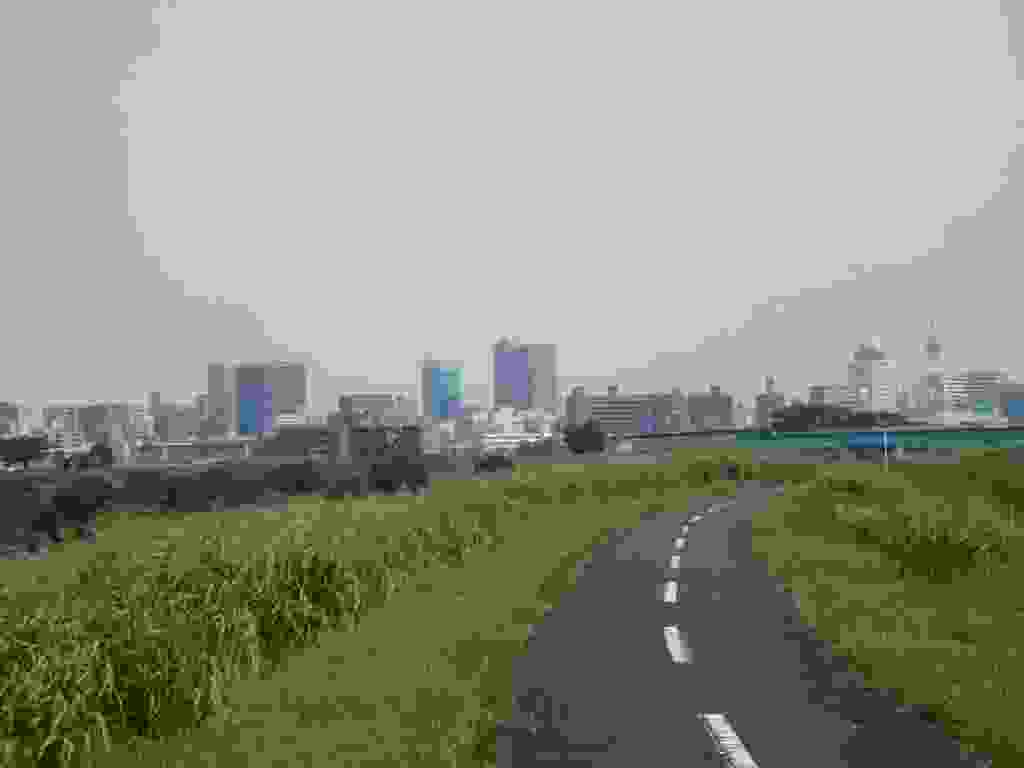
\includegraphics[width=\mywidth]{../wp-content/uploads/2015/08/P7255627-1024x768.jpg} } 
 \newline
 \newline
\centerline{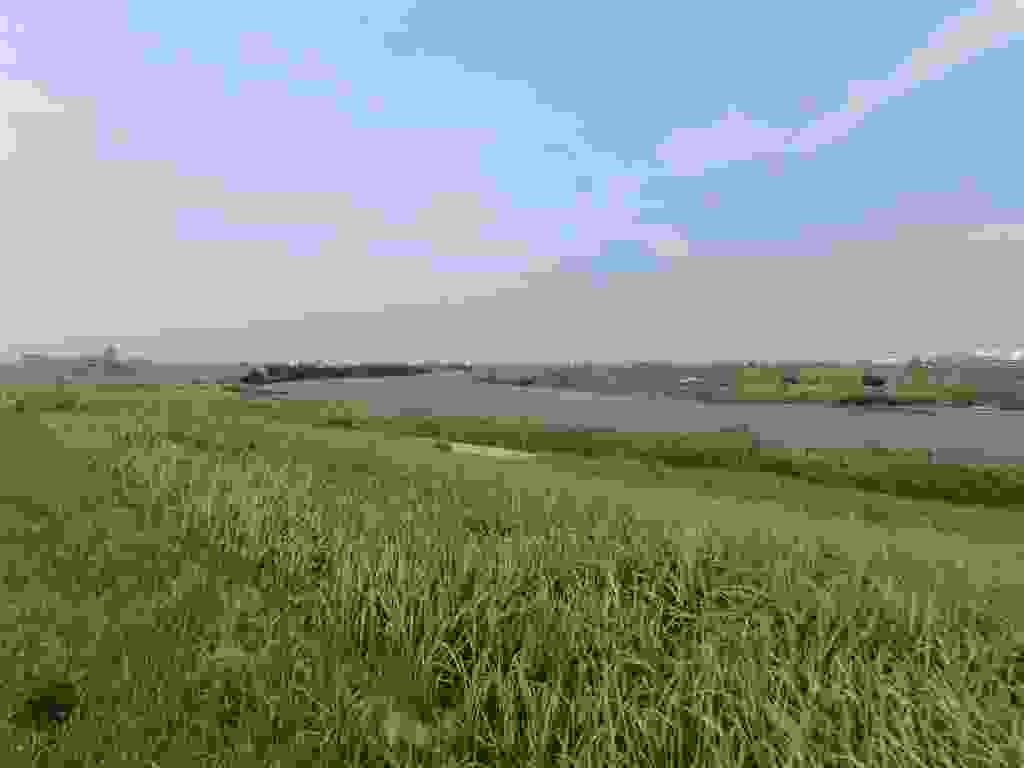
\includegraphics[width=\mywidth]{../wp-content/uploads/2015/08/P7255626-1024x768.jpg} } 
 \newline
 \newline
\centerline{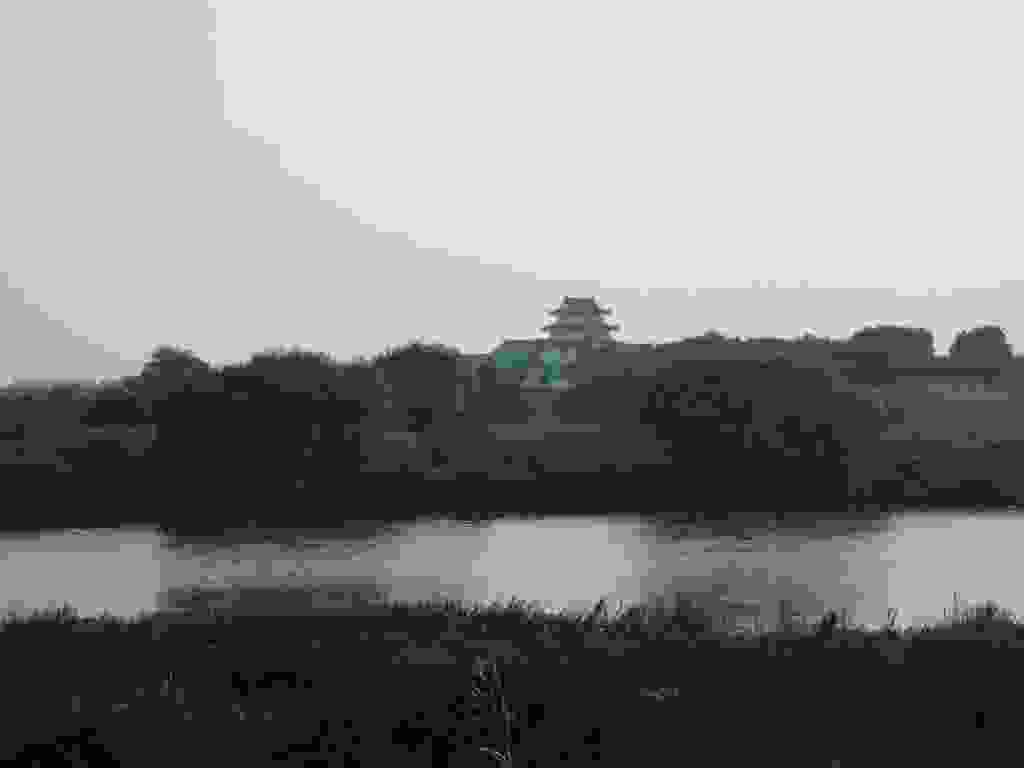
\includegraphics[width=\mywidth]{../wp-content/uploads/2015/08/P7255632-1024x768.jpg} } 
 \newline
 \newline
\centerline{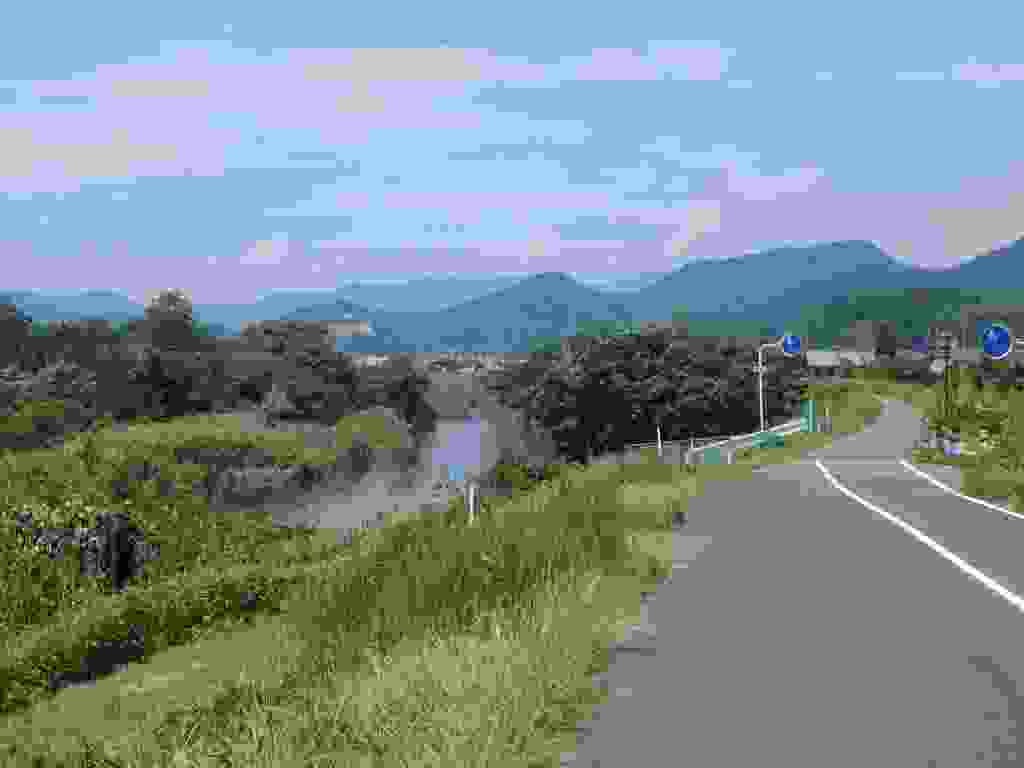
\includegraphics[width=\mywidth]{../wp-content/uploads/2015/08/P7265654-1024x768.jpg} } 
 \newline
 Le Japon est tellement sur que je peux camper un peu partout. \newline
 \newline
\centerline{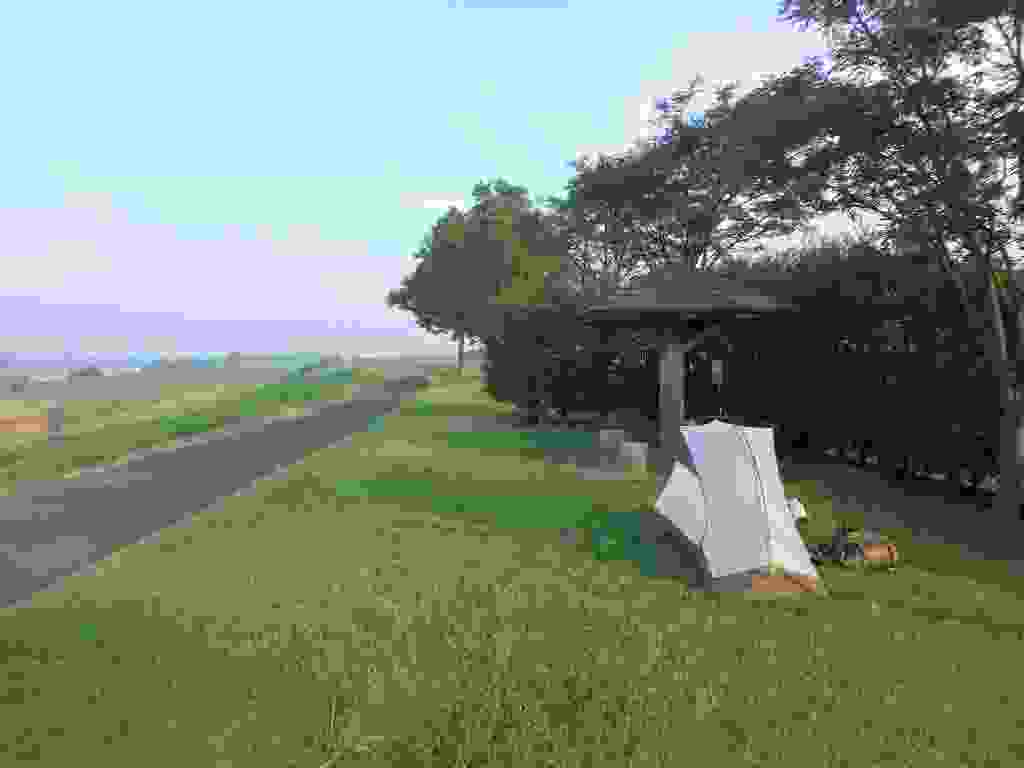
\includegraphics[width=\mywidth]{../wp-content/uploads/2015/08/P7265649-1024x768.jpg} } 
 \newline
 Festival dans une ville ou je me suis arreté pour une soirée, avec un concert de jazz \newline
 \newline
\centerline{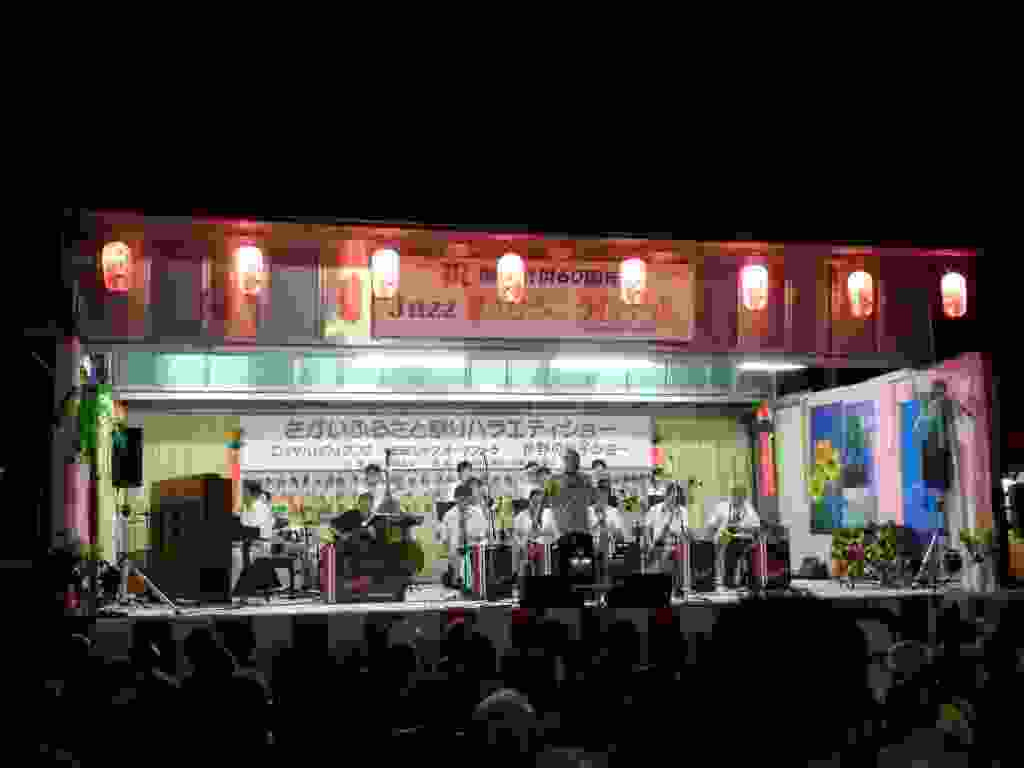
\includegraphics[width=\mywidth]{../wp-content/uploads/2015/08/P7255643-1024x768.jpg} } 
 \newline
 Et un spectacle de hip hop par des enfants, très fun ! \newline
 \newline
\centerline{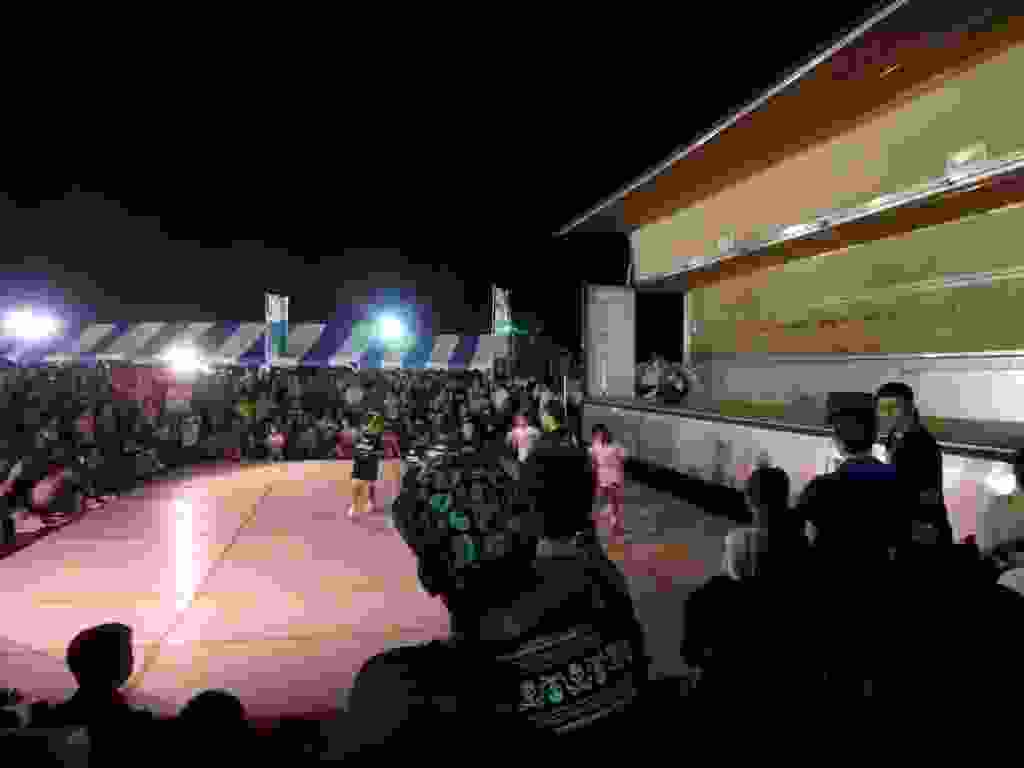
\includegraphics[width=\mywidth]{../wp-content/uploads/2015/08/P7255645-1024x768.jpg} } 
 \newline
 La route commence à s'élever, camping au bord d'un lac \newline
 \newline
\centerline{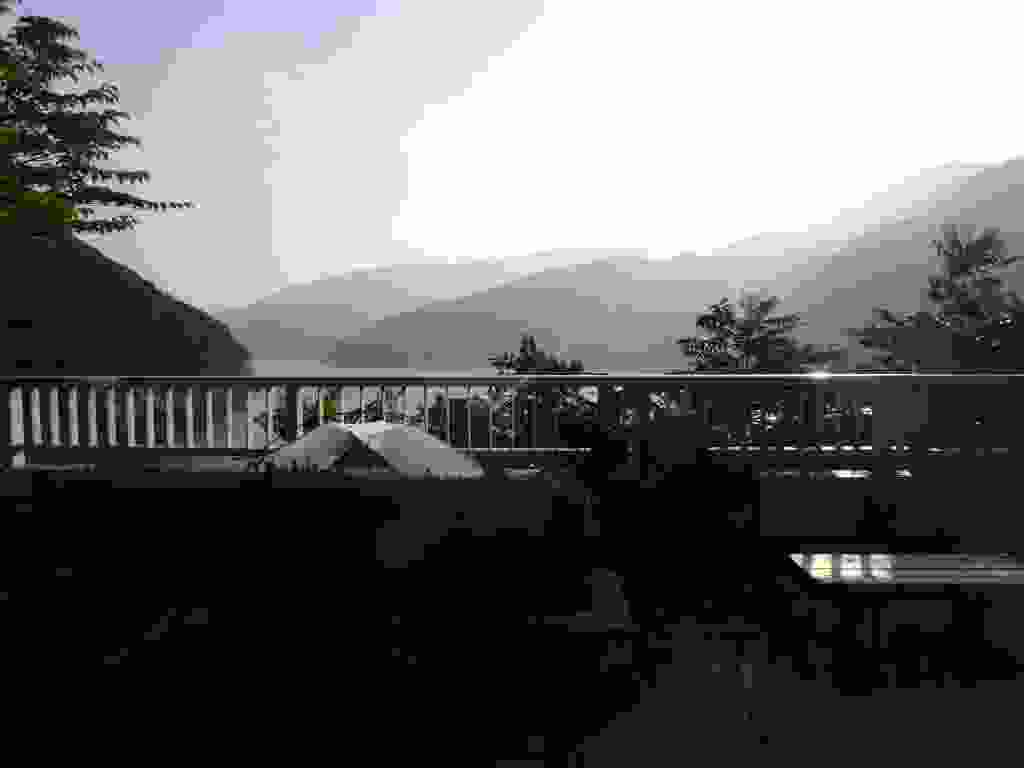
\includegraphics[width=\mywidth]{../wp-content/uploads/2015/08/P7275663-1024x768.jpg} } 
 \newline
 \newline
\centerline{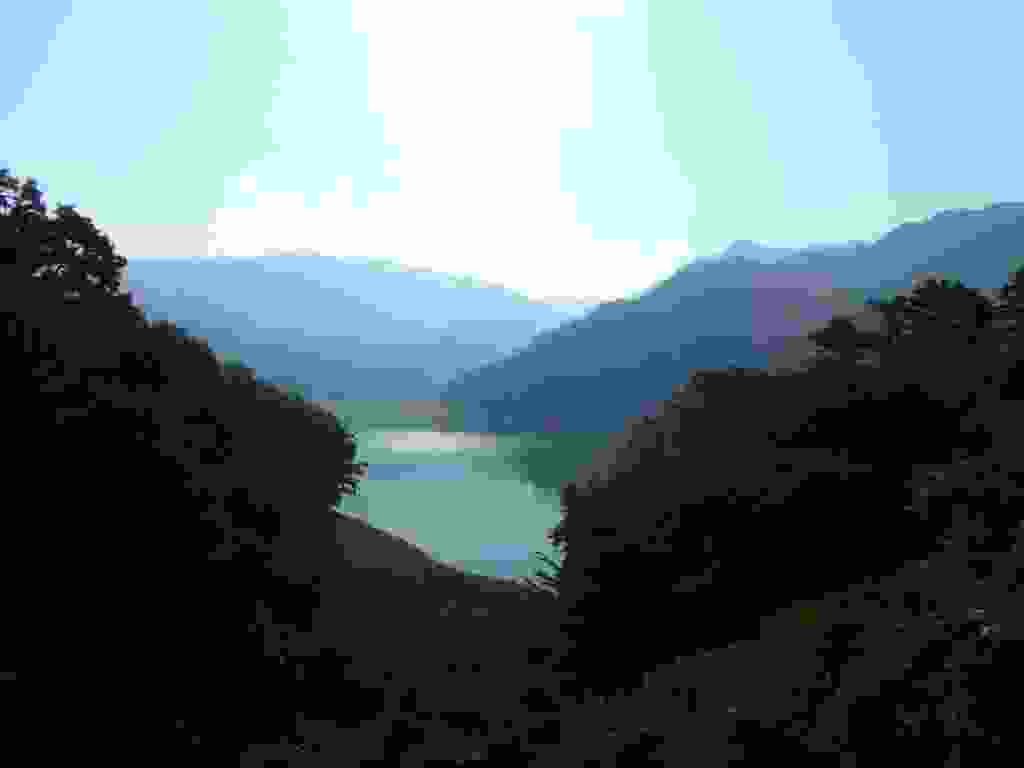
\includegraphics[width=\mywidth]{../wp-content/uploads/2015/08/P7275665-1024x768.jpg} } 
 \newline
 \newline
\centerline{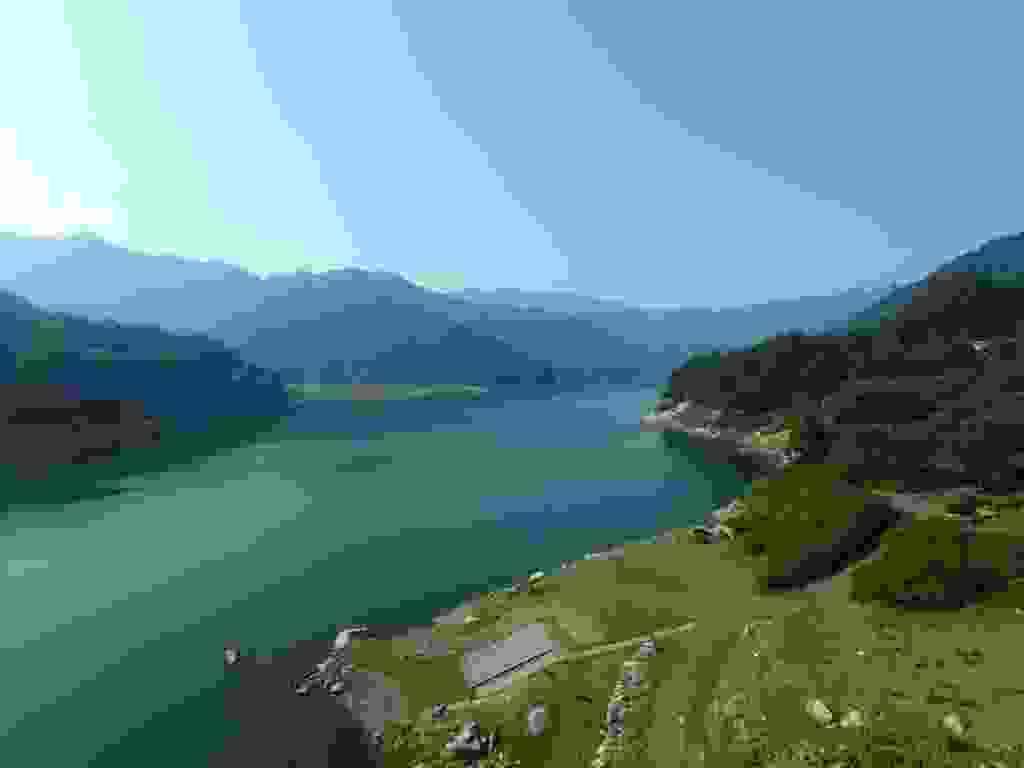
\includegraphics[width=\mywidth]{../wp-content/uploads/2015/08/P7275667-1024x768.jpg} } 
 \newline
 \newline
\centerline{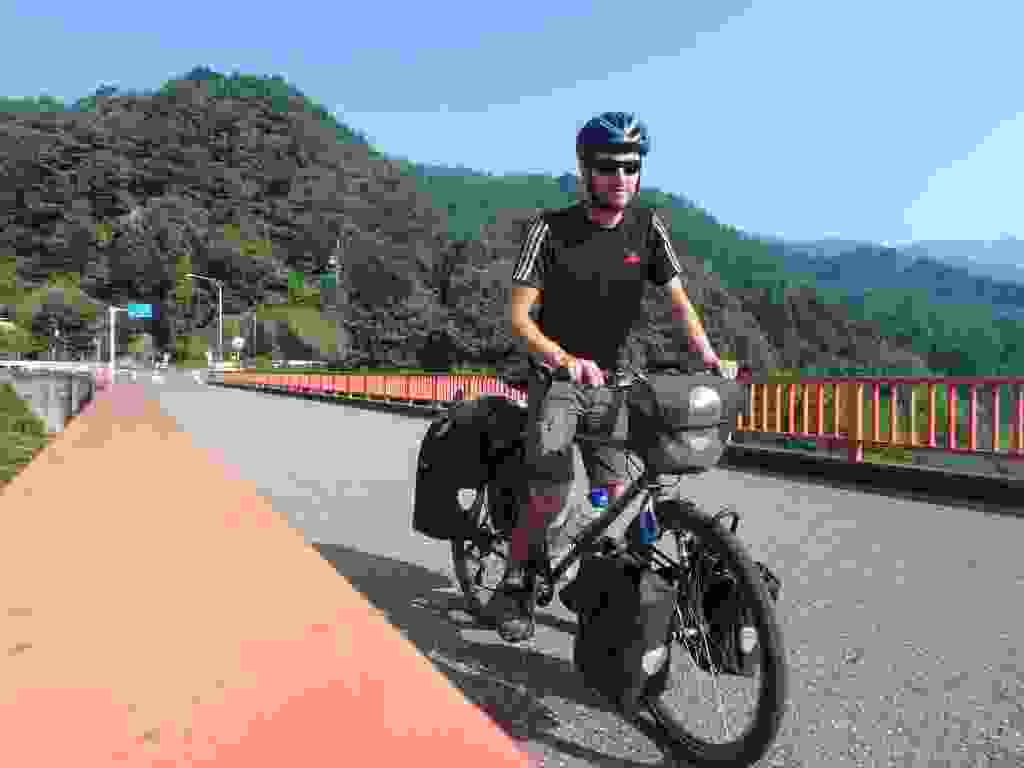
\includegraphics[width=\mywidth]{../wp-content/uploads/2015/08/P7275668-1024x768.jpg} } 
 \newline
 Au sommet d'un col je croise des singes \newline
 \newline
\centerline{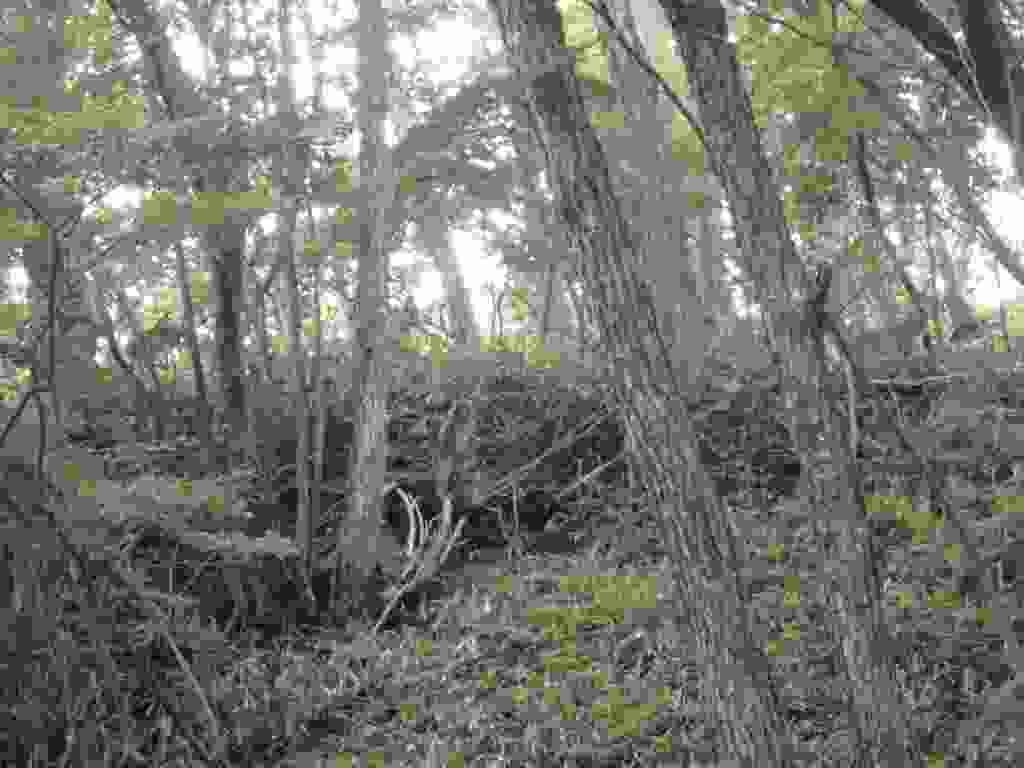
\includegraphics[width=\mywidth]{../wp-content/uploads/2015/08/P7275672-1024x768.jpg} } 
 \newline
 J'arrive à Nikko, célèbre pour ses temples et shrines inscrits au patrimoine de l'Unesco. \newline
 \newline
\centerline{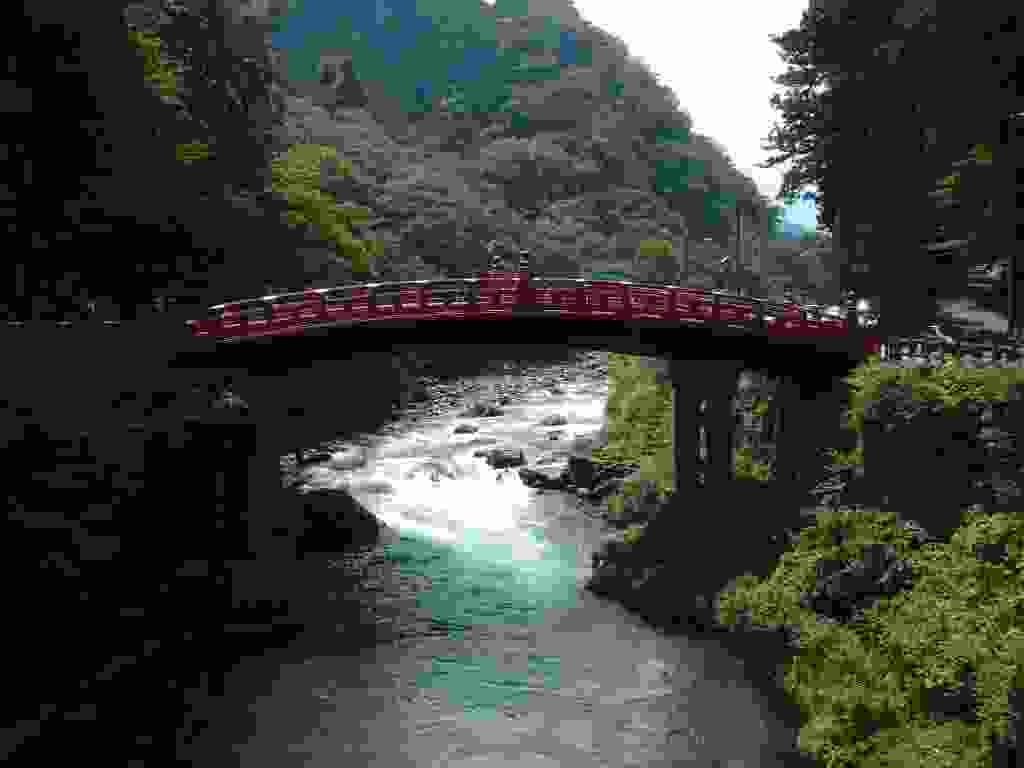
\includegraphics[width=\mywidth]{../wp-content/uploads/2015/08/P7275678-1024x768.jpg} } 
 \newline
 \newline
\centerline{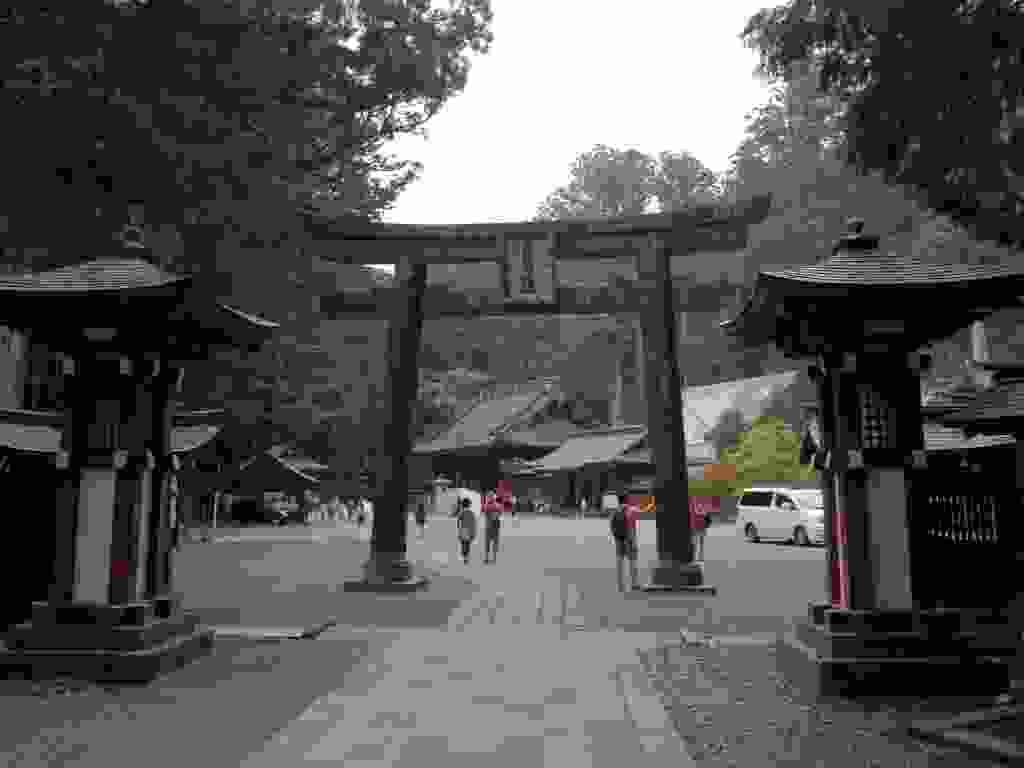
\includegraphics[width=\mywidth]{../wp-content/uploads/2015/08/P7285733-1024x768.jpg} } 
 \newline
 Beaucoup de groupe d'enfants japonais visitent Nikko, des jeunes viennent me poser des questions pour s'exercer en anglais. \newline
 \newline
\centerline{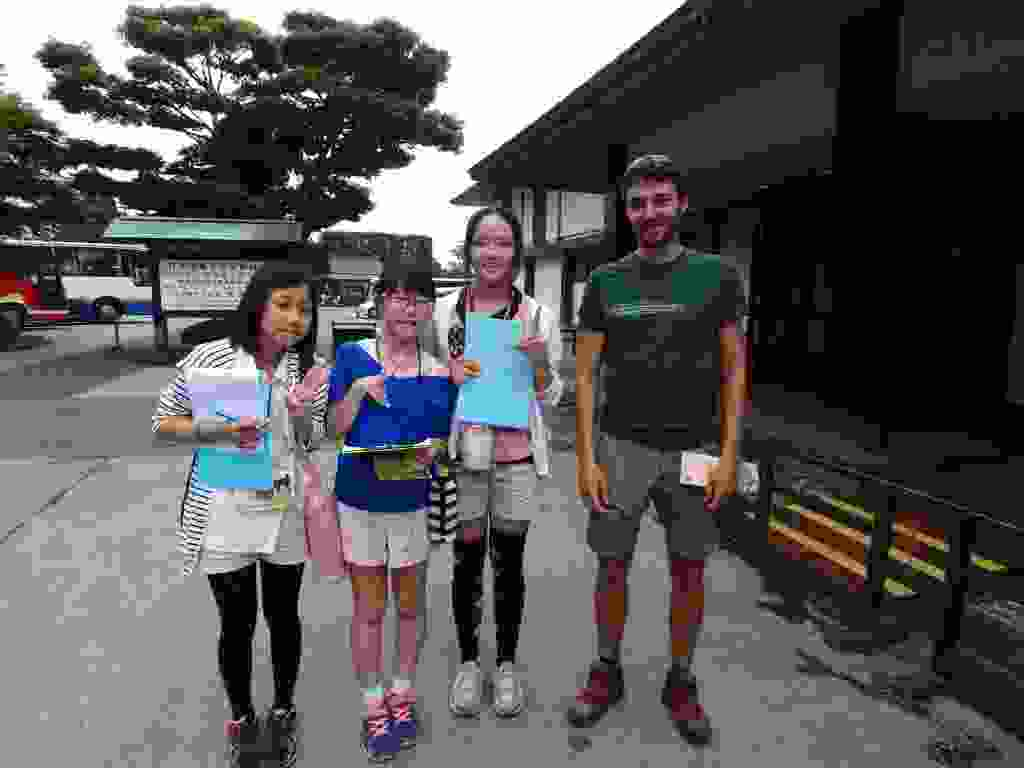
\includegraphics[width=\mywidth]{../wp-content/uploads/2015/08/P7285692-1024x768.jpg} } 
 \newline
 Le temple de Toshogu avec le mausolée du Shogun Tokugawa Ieyasu. \newline
 \newline
\centerline{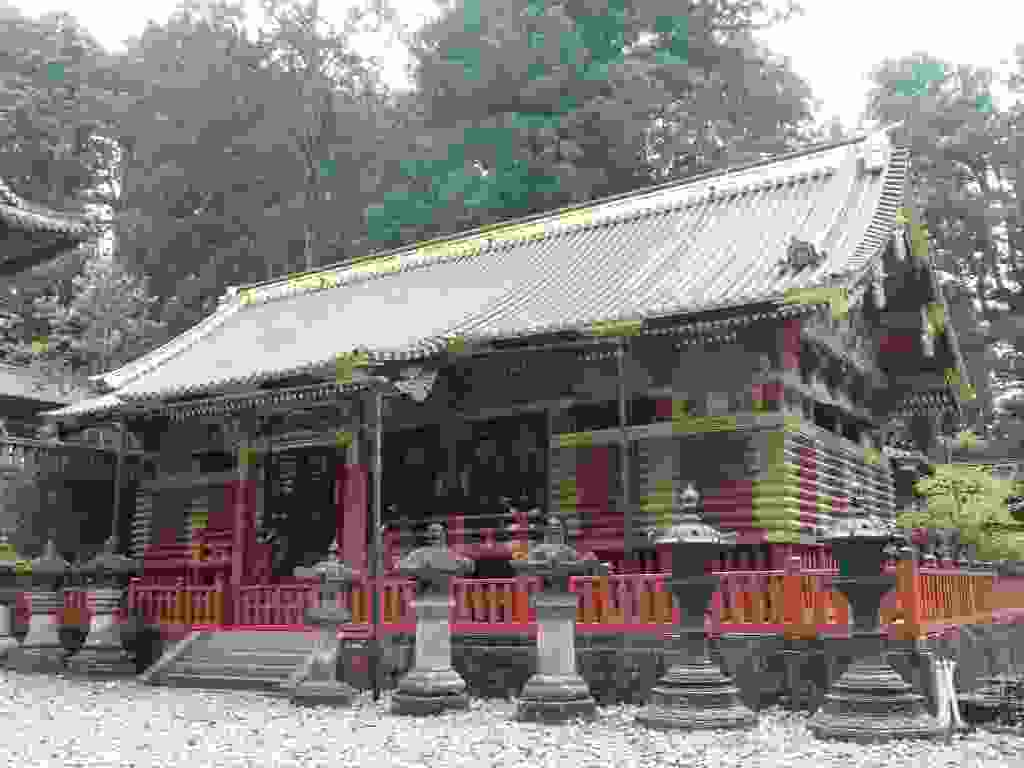
\includegraphics[width=\mywidth]{../wp-content/uploads/2015/08/P7285706-1024x768.jpg} } 
 \newline
 \newline
\centerline{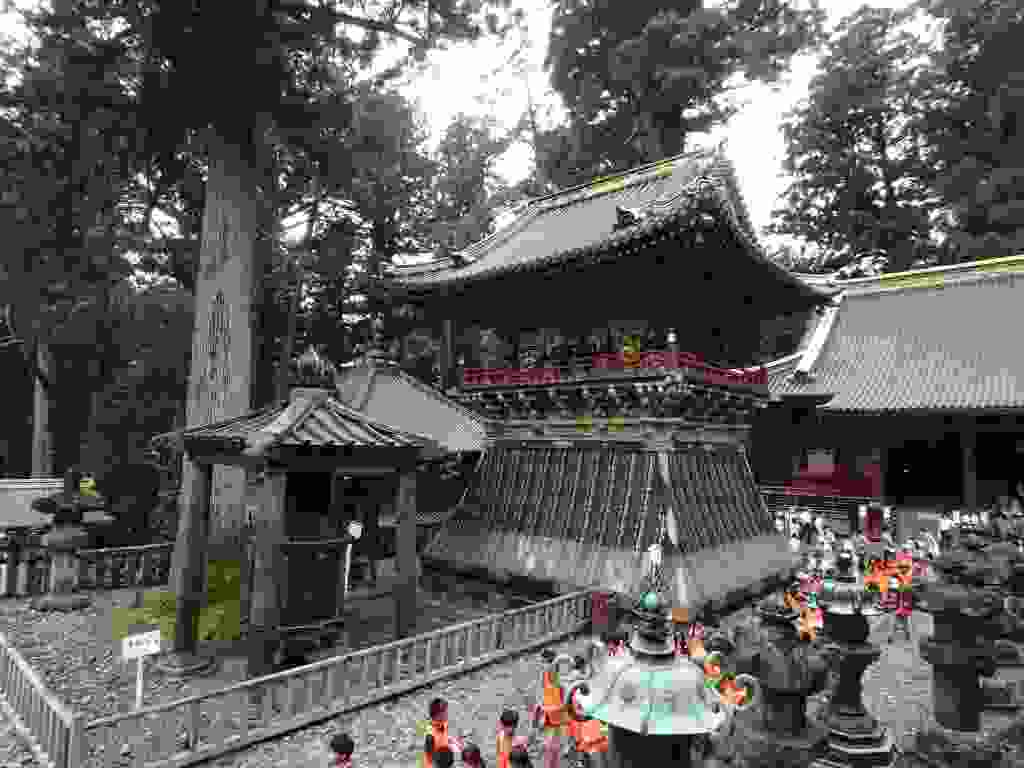
\includegraphics[width=\mywidth]{../wp-content/uploads/2015/08/P7285727-1024x768.jpg} } 
 \newline
 \newline
\centerline{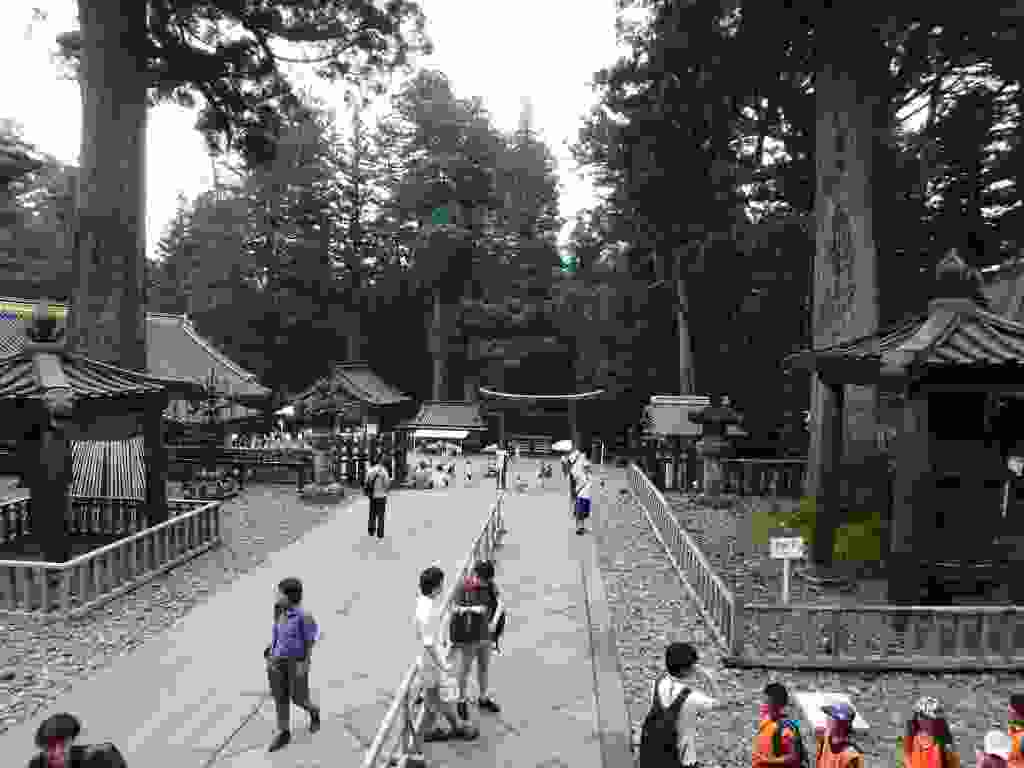
\includegraphics[width=\mywidth]{../wp-content/uploads/2015/08/P7285726-1024x768.jpg} } 
 \newline
 \newline
\centerline{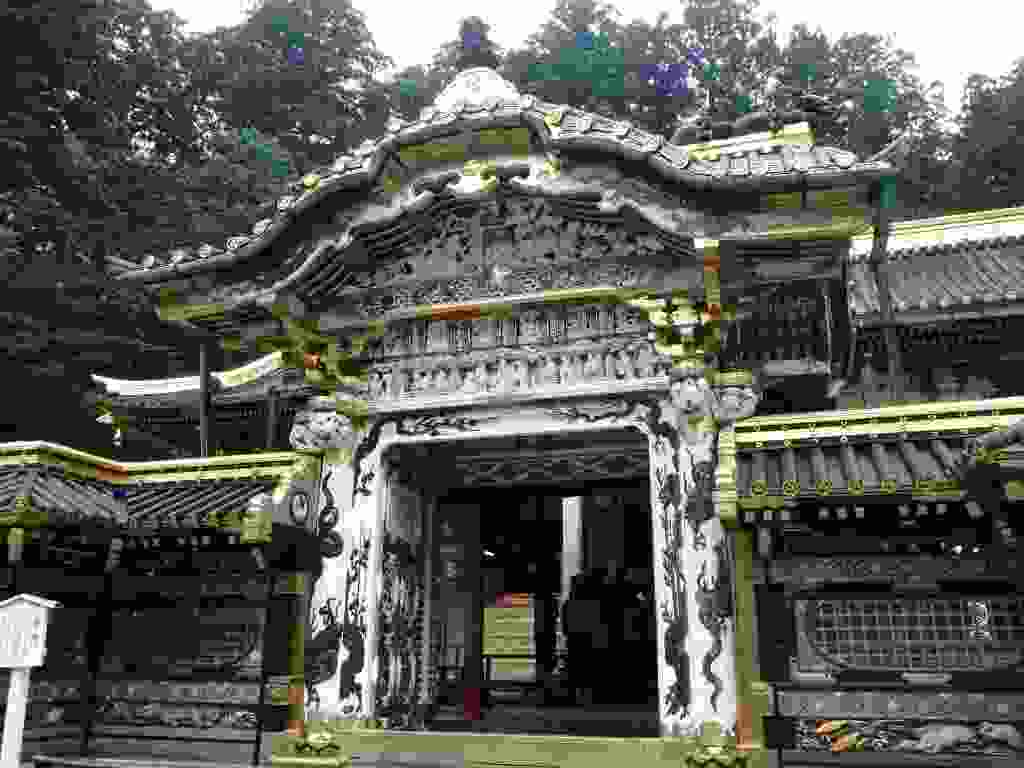
\includegraphics[width=\mywidth]{../wp-content/uploads/2015/08/P7285724-1024x768.jpg} } 
 \newline
 Représentation des 3 singes sages : « Ne rien voir, ne rien entendre, ne rien dire » \newline
 \newline
\centerline{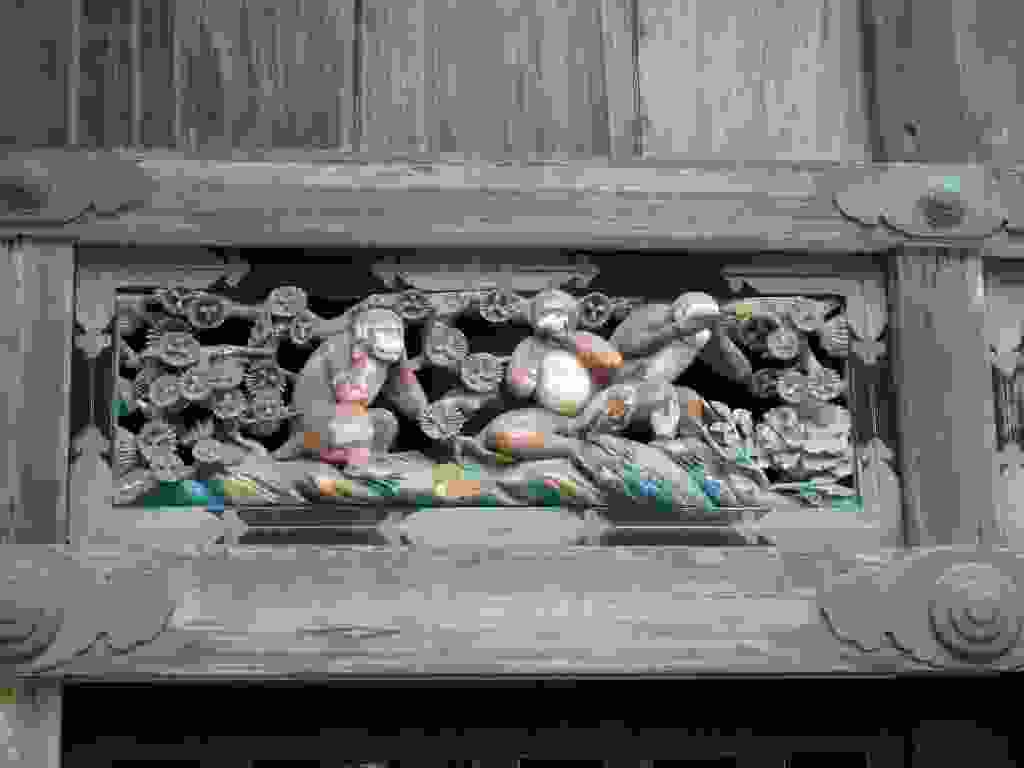
\includegraphics[width=\mywidth]{../wp-content/uploads/2015/08/P7285703-1024x768.jpg} } 
 \newline
 Le shrine de Taiyuin \newline
 \newline
\centerline{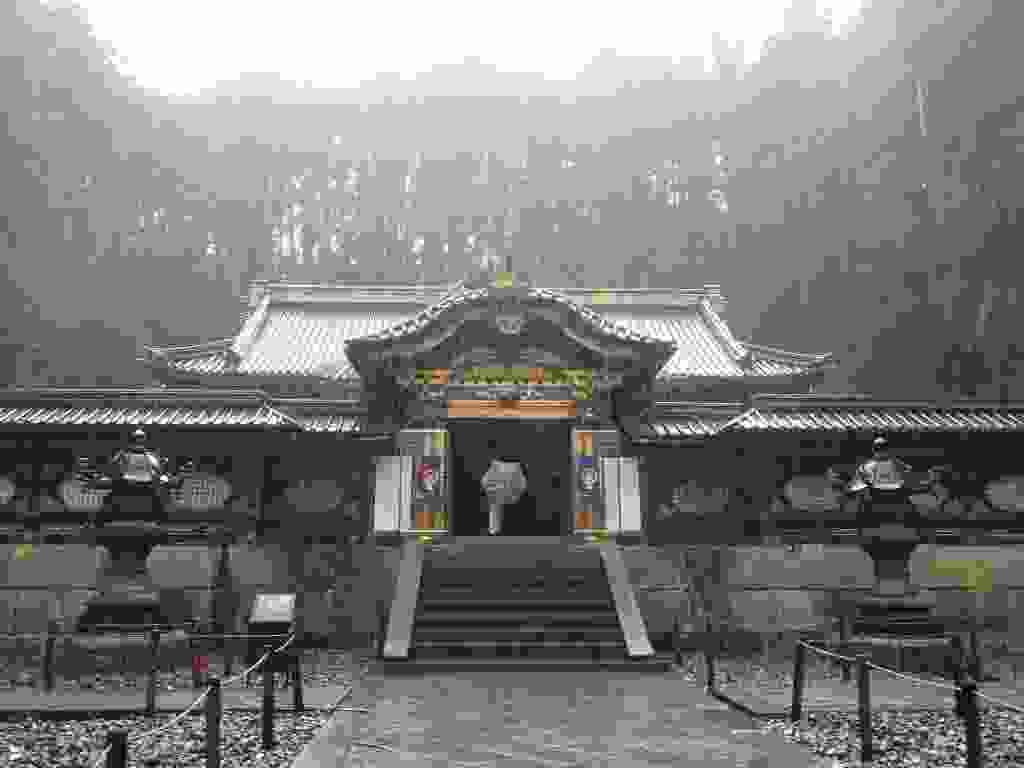
\includegraphics[width=\mywidth]{../wp-content/uploads/2015/08/P7285745-1024x768.jpg} } 
 \newline
 Un chemin dans la foret permet d'accéder à un petit shrine \newline
 \newline
\centerline{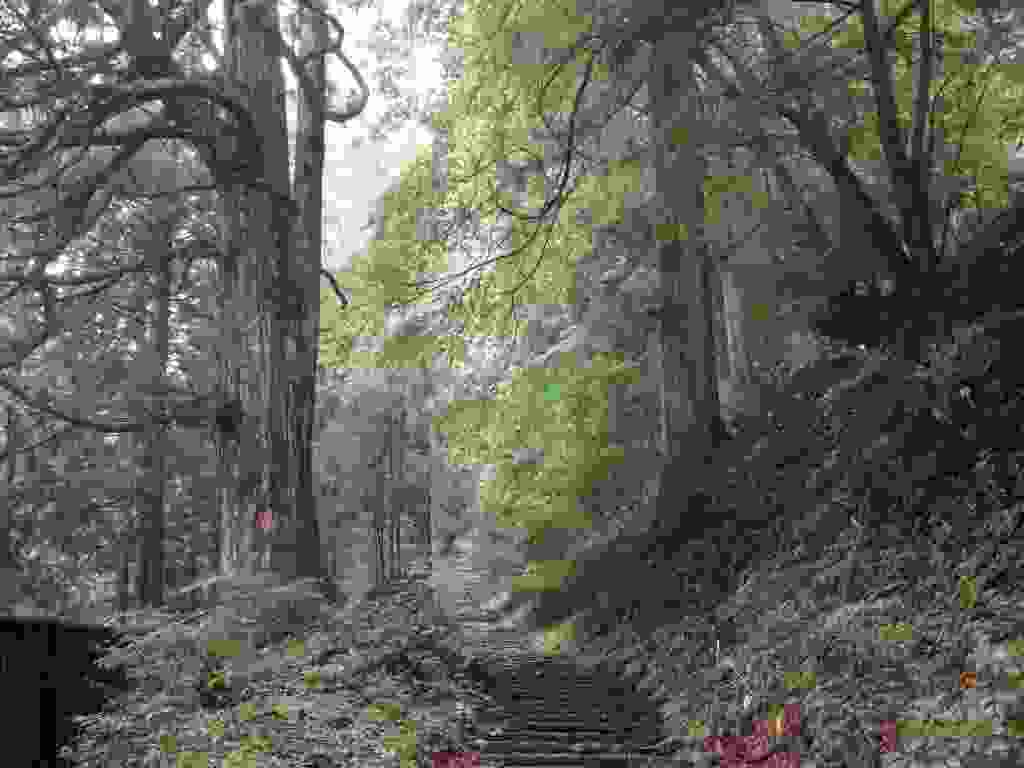
\includegraphics[width=\mywidth]{../wp-content/uploads/2015/08/P7285754-1024x768.jpg} } 
 \newline
 \newline
\centerline{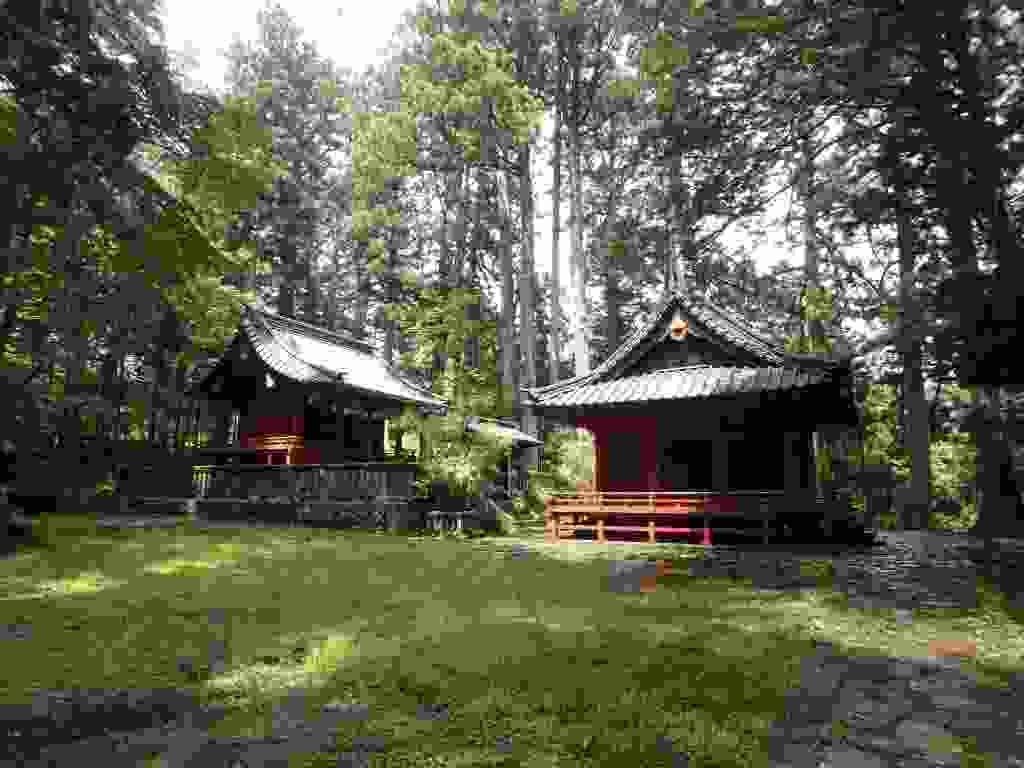
\includegraphics[width=\mywidth]{../wp-content/uploads/2015/08/P7285760-1024x768.jpg} } 
 \newline
 Un alignement impressionnant de Jizo, des protecteurs \newline
 \newline
\centerline{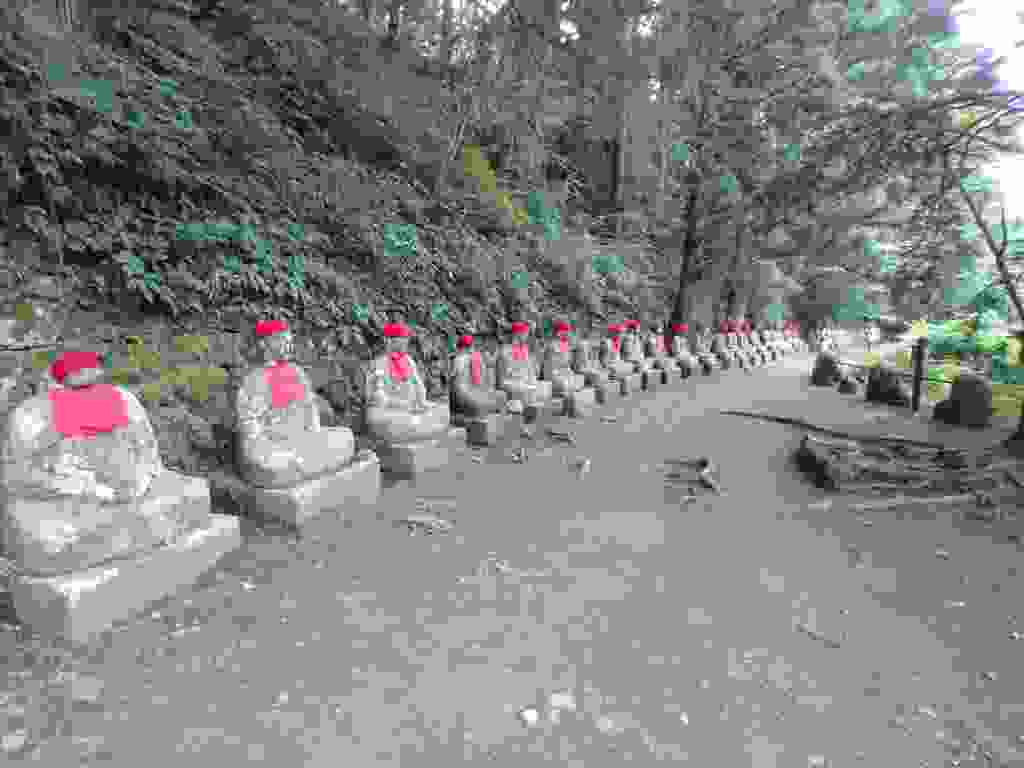
\includegraphics[width=\mywidth]{../wp-content/uploads/2015/08/P7275684-1024x768.jpg} } 
 \newline
 \newline
\centerline{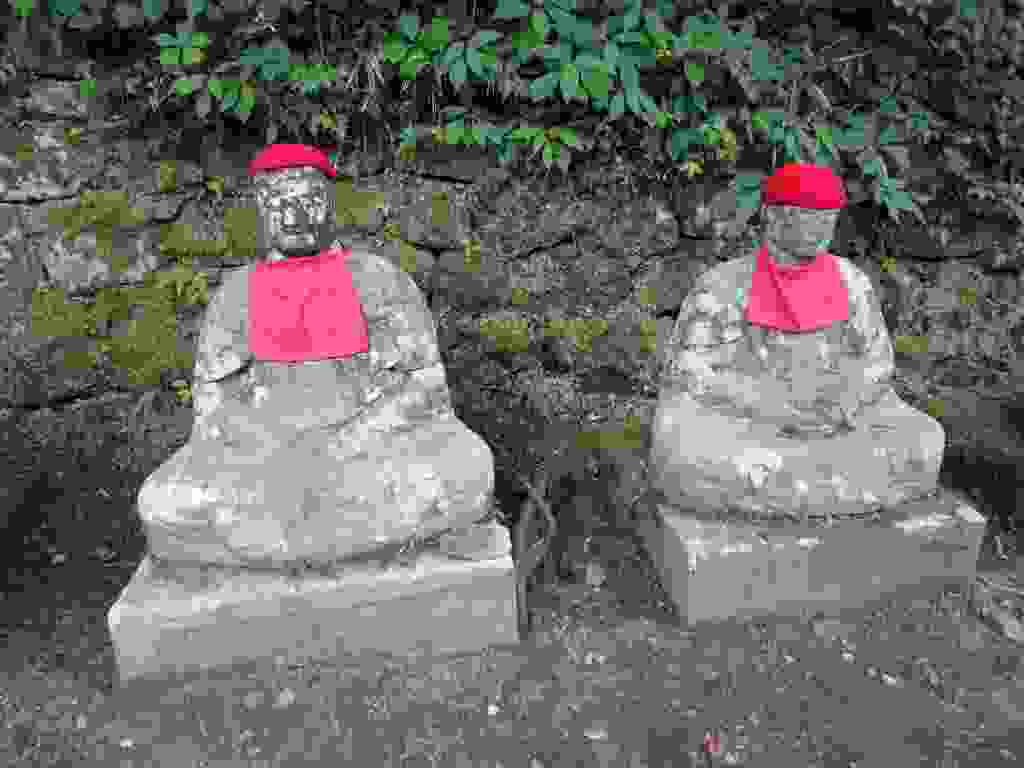
\includegraphics[width=\mywidth]{../wp-content/uploads/2015/08/P7275685-1024x768.jpg} } 
 \newline
 Je repars vers le parc national de Nikko \newline
 \newline
\centerline{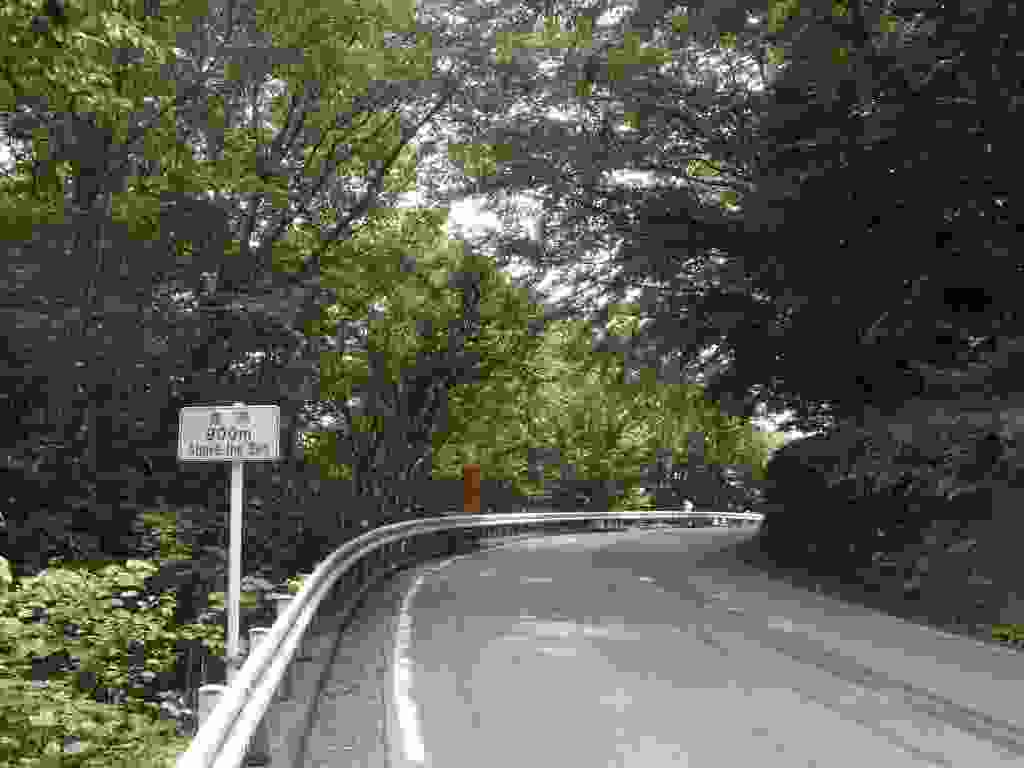
\includegraphics[width=\mywidth]{../wp-content/uploads/2015/08/P7295772-1024x768.jpg} } 
 \newline
 \newline
\centerline{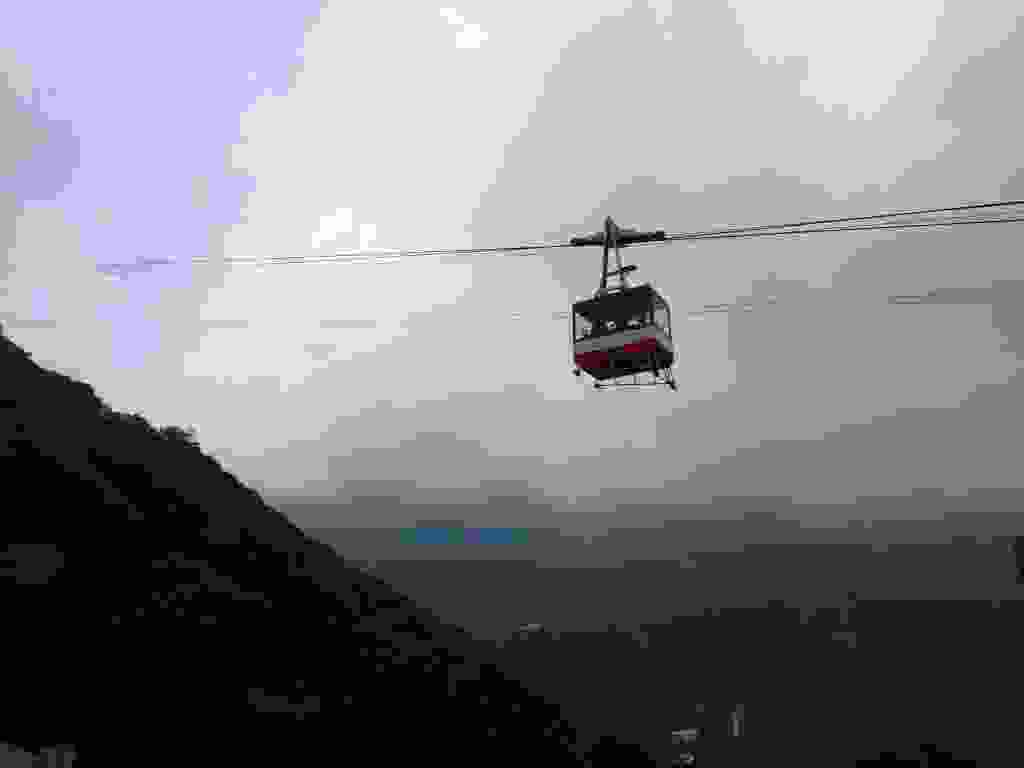
\includegraphics[width=\mywidth]{../wp-content/uploads/2015/08/P7295774-1024x768.jpg} } 
 \newline
 La cascade de Kegon \newline
 \newline
\centerline{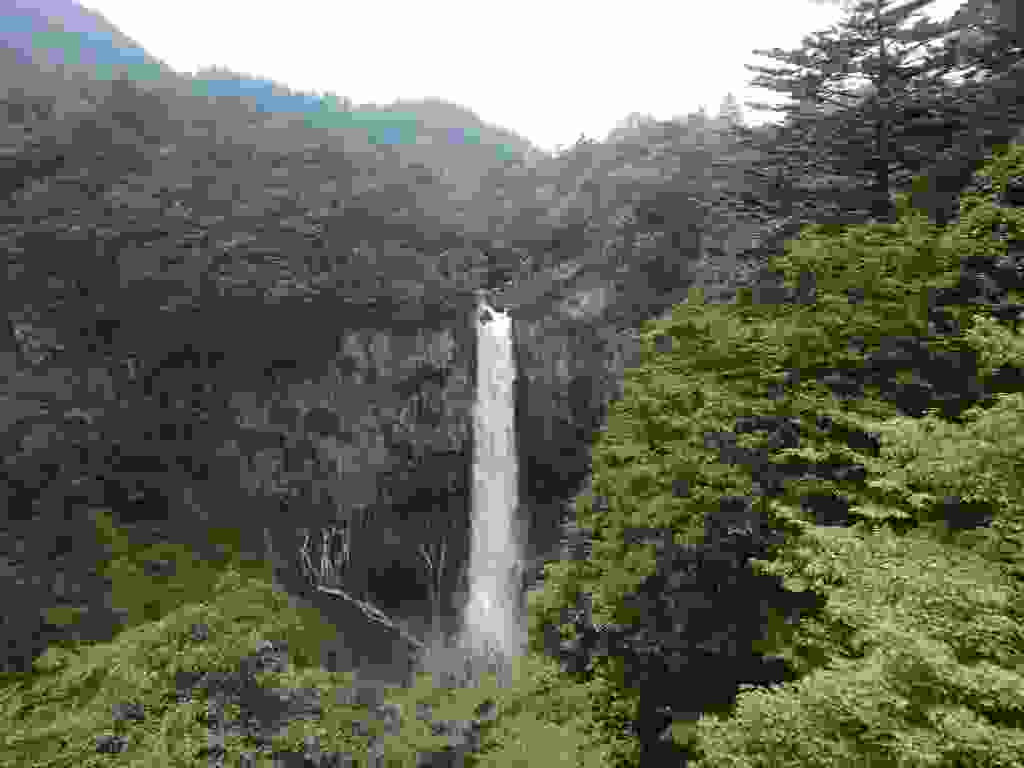
\includegraphics[width=\mywidth]{../wp-content/uploads/2015/08/P7295778-1024x768.jpg} } 
 \newline
 Balade pour voir le lac Chūzenji, avec un temps pas idéal. \newline
 \newline
\centerline{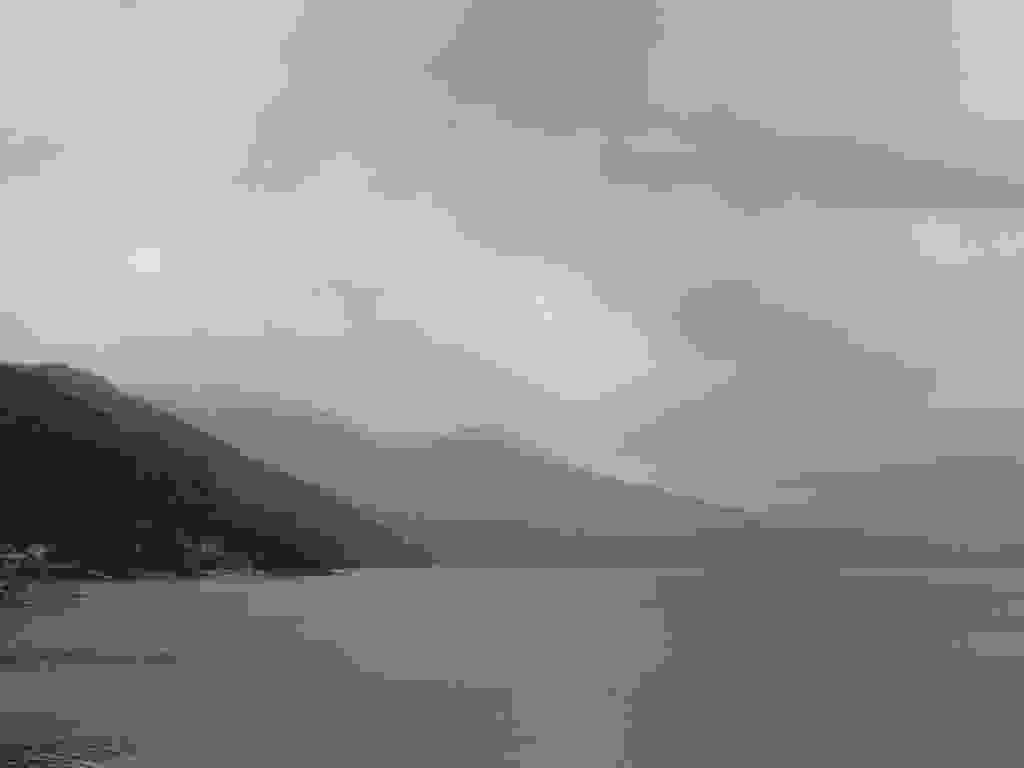
\includegraphics[width=\mywidth]{../wp-content/uploads/2015/08/P7295782-1024x768.jpg} } 
 \newline
 \newline
\centerline{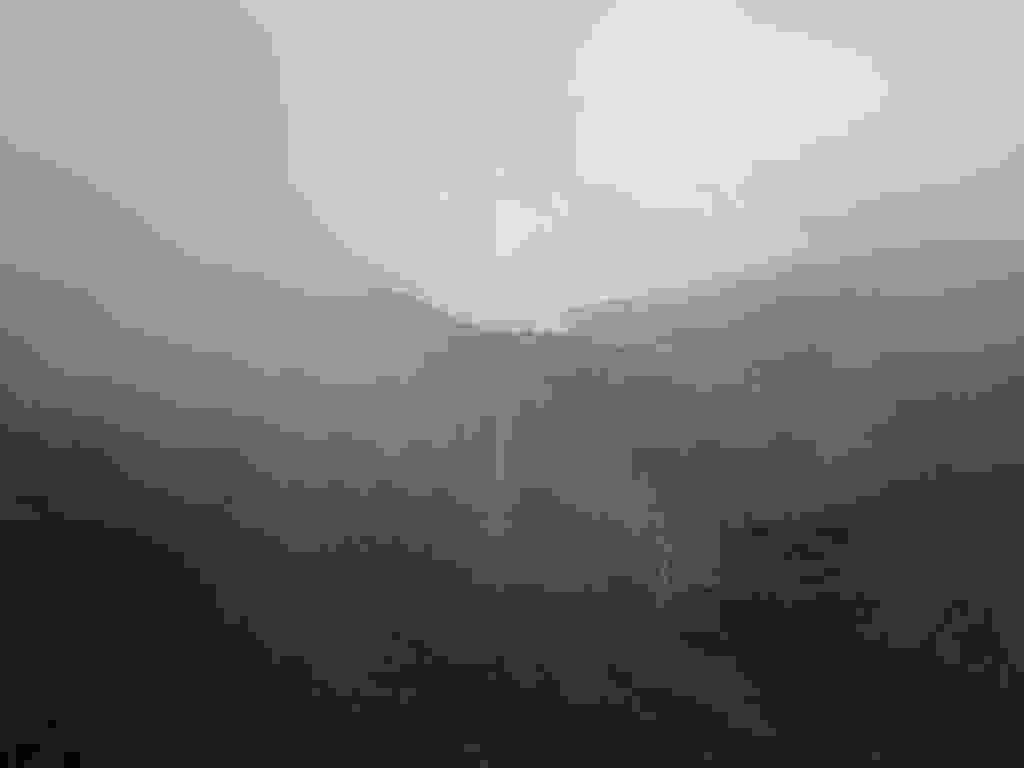
\includegraphics[width=\mywidth]{../wp-content/uploads/2015/08/P7295791-1024x768.jpg} } 
 \newline
 Je continue la montée jusqu'à la cascade et au lac de Yumoto. \newline
 \newline
\centerline{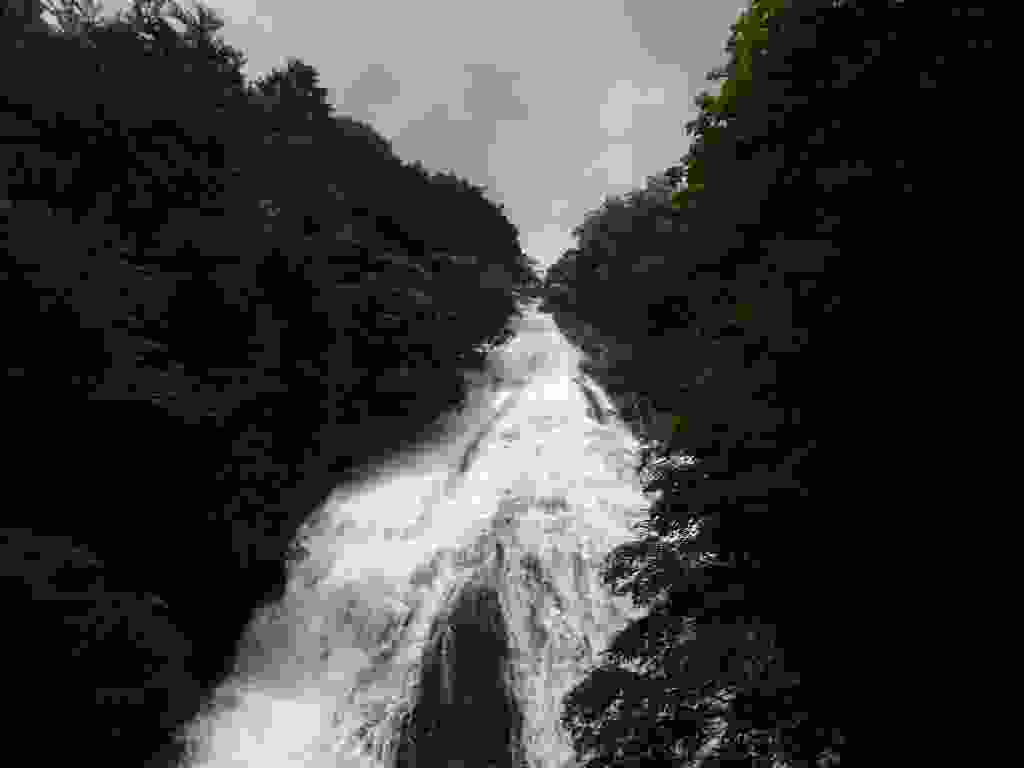
\includegraphics[width=\mywidth]{../wp-content/uploads/2015/08/P7305824-1024x768.jpg} } 
 \newline
 \newline
\centerline{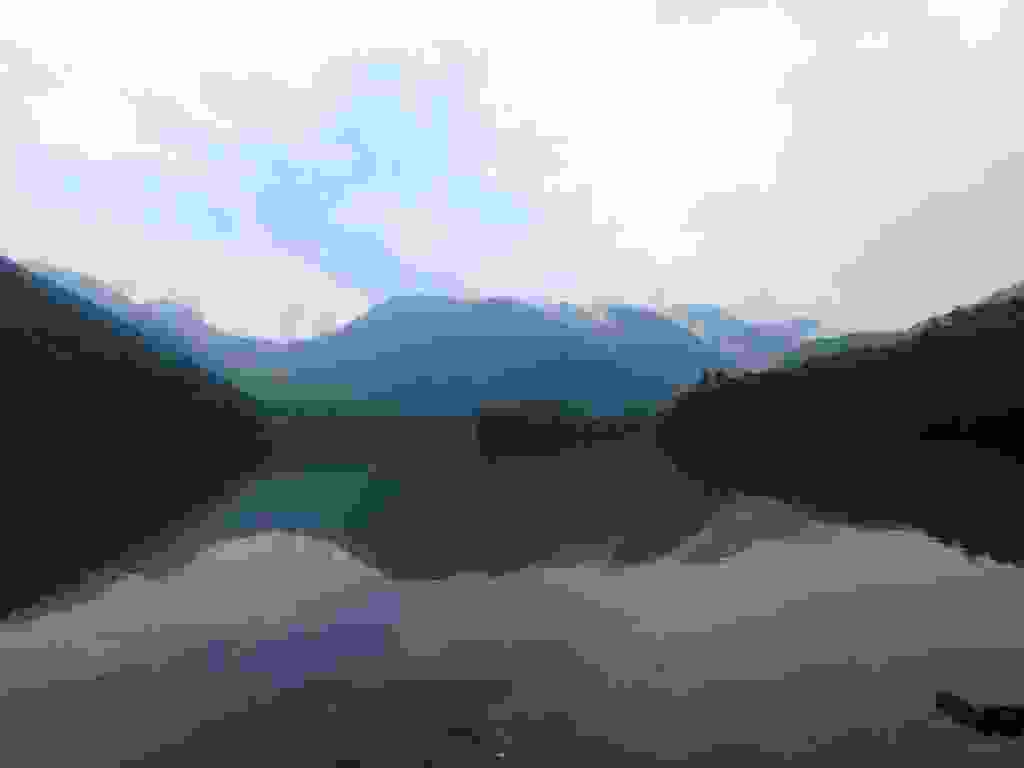
\includegraphics[width=\mywidth]{../wp-content/uploads/2015/08/P7305825-1024x768.jpg} } 
 \newline
 \newline
\centerline{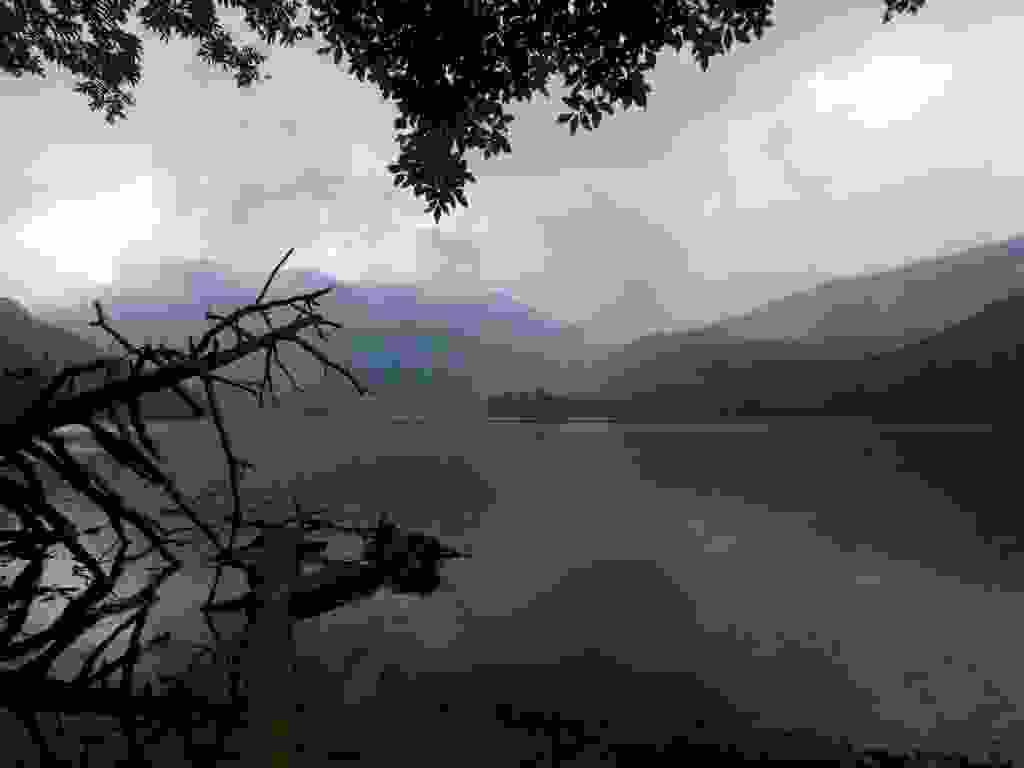
\includegraphics[width=\mywidth]{../wp-content/uploads/2015/08/P7305820-1024x768.jpg} } 
 \newline
 Yumoto est aussi connu pour ses onsen, ou sources chaudes \newline
 \newline
\centerline{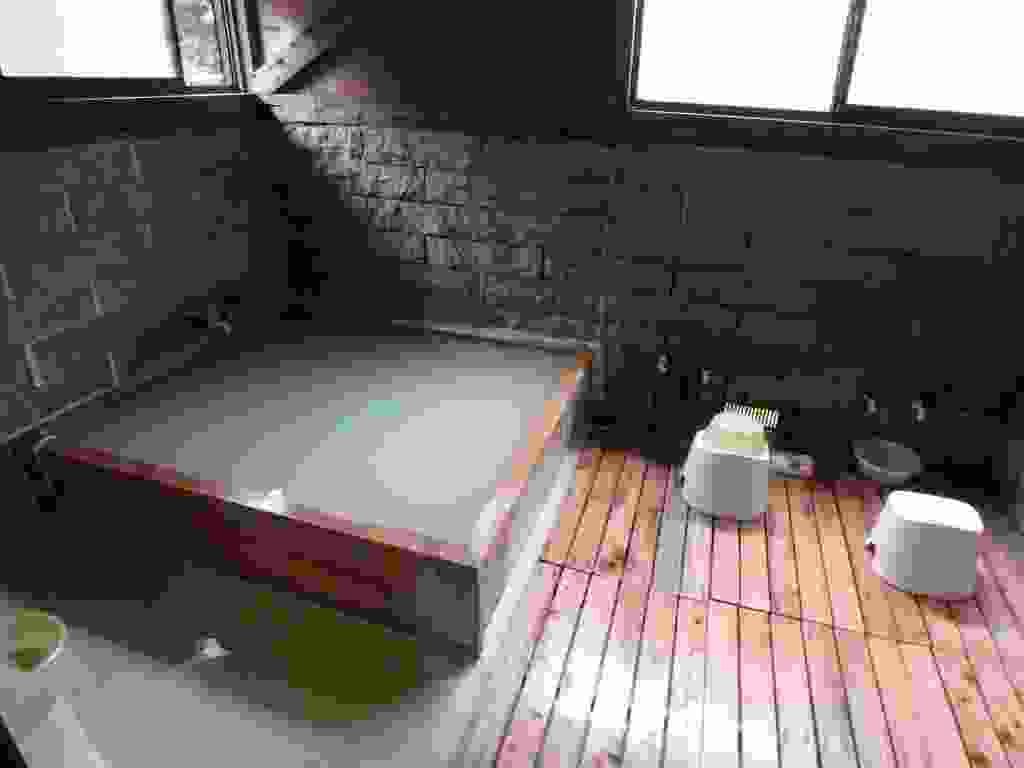
\includegraphics[width=\mywidth]{../wp-content/uploads/2015/08/P7305829-1024x768.jpg} } 
 \newline
 Je passe ensuite le col de Konsei à plus de 2000m \newline
 \newline
\centerline{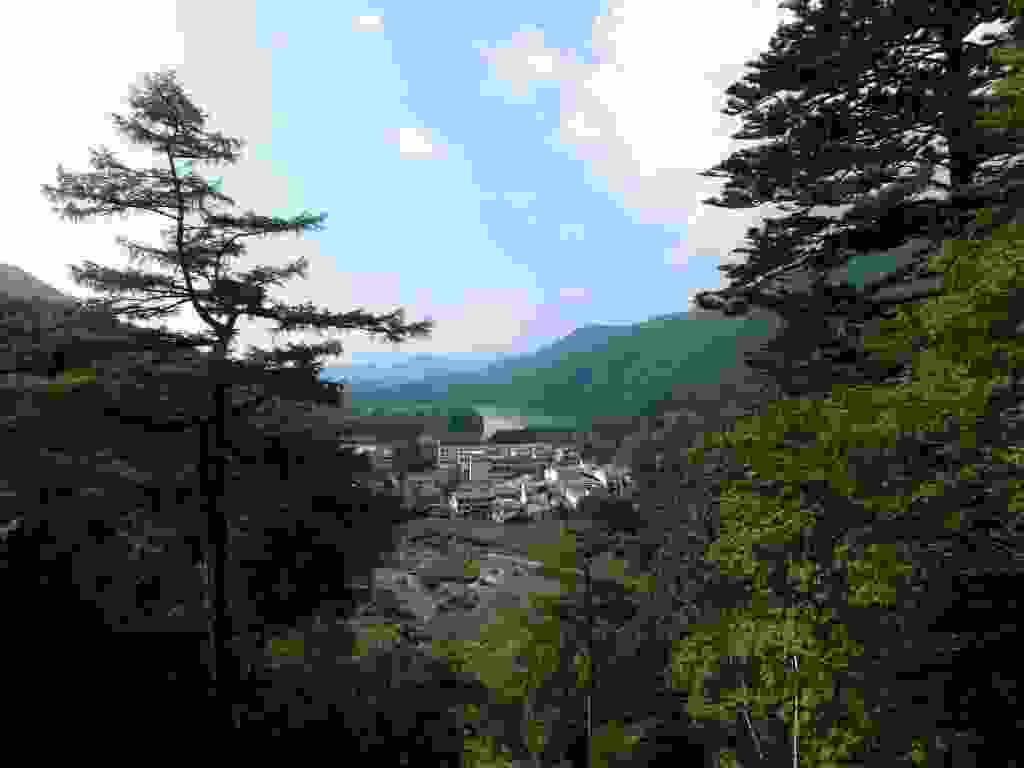
\includegraphics[width=\mywidth]{../wp-content/uploads/2015/08/P7315831-1024x768.jpg} } 
 \newline
 \newline
\centerline{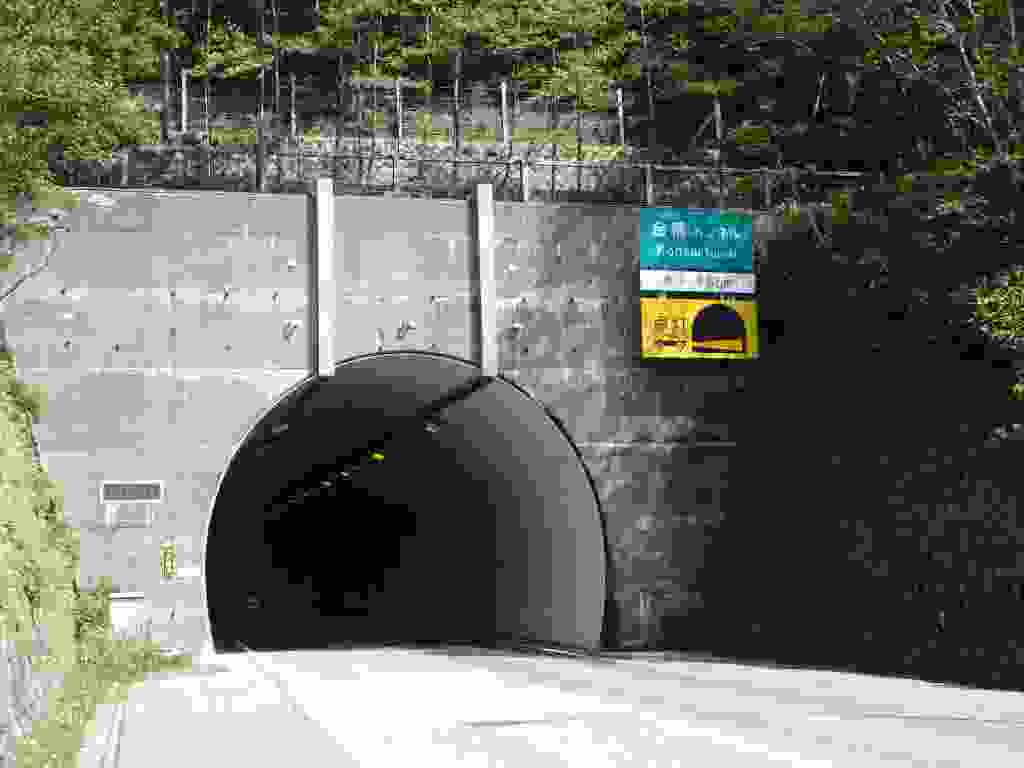
\includegraphics[width=\mywidth]{../wp-content/uploads/2015/08/P7315837-1024x768.jpg} } 
 \newline
 \newline
\centerline{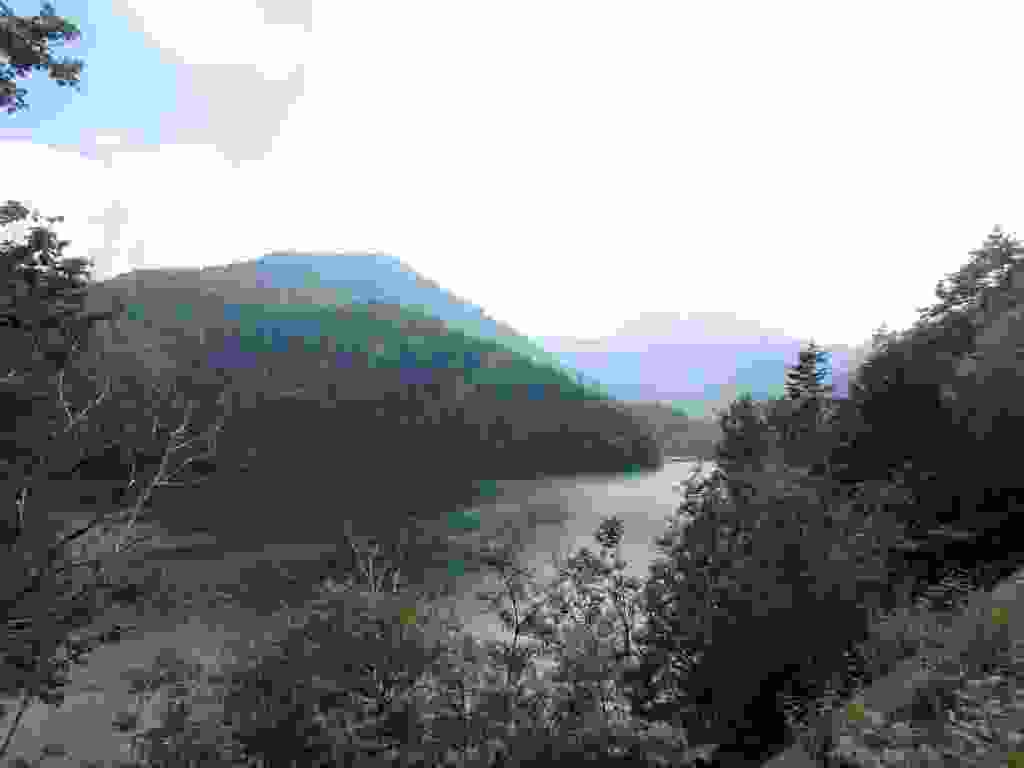
\includegraphics[width=\mywidth]{../wp-content/uploads/2015/08/P7315838-1024x768.jpg} } 
 \newline
 Je croise une station de ski, l'envie me prend de faire quelques descentes. \newline
 \newline
\centerline{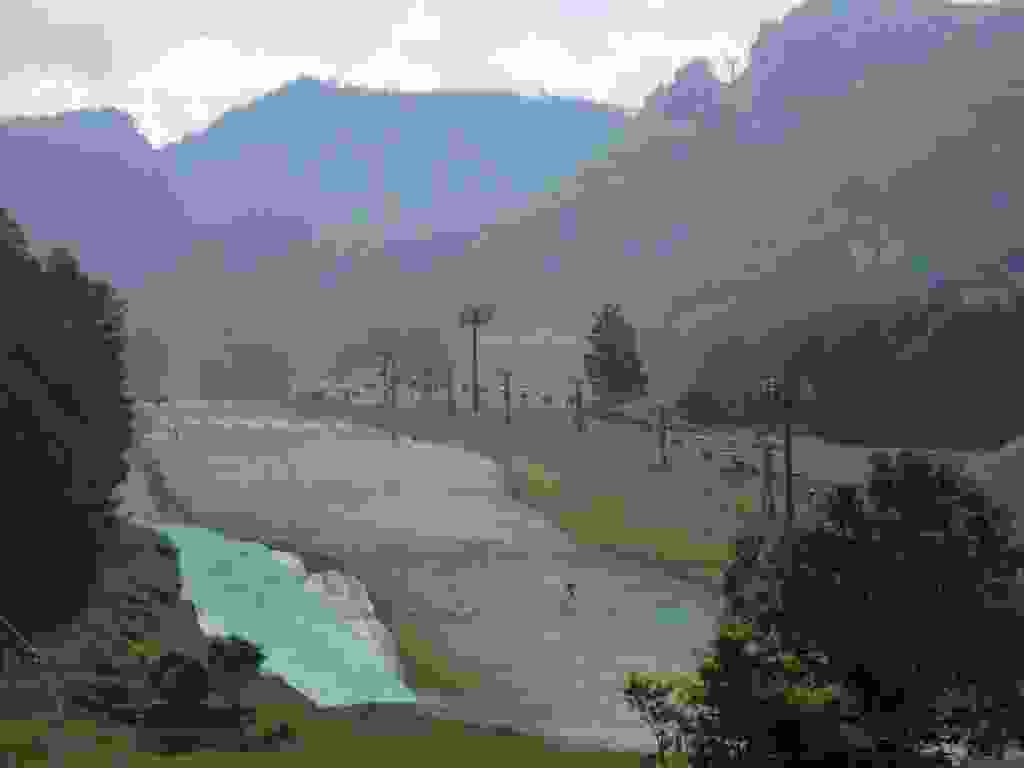
\includegraphics[width=\mywidth]{../wp-content/uploads/2015/08/P7315840-1024x768.jpg} } 
 \newline
 \newline
\centerline{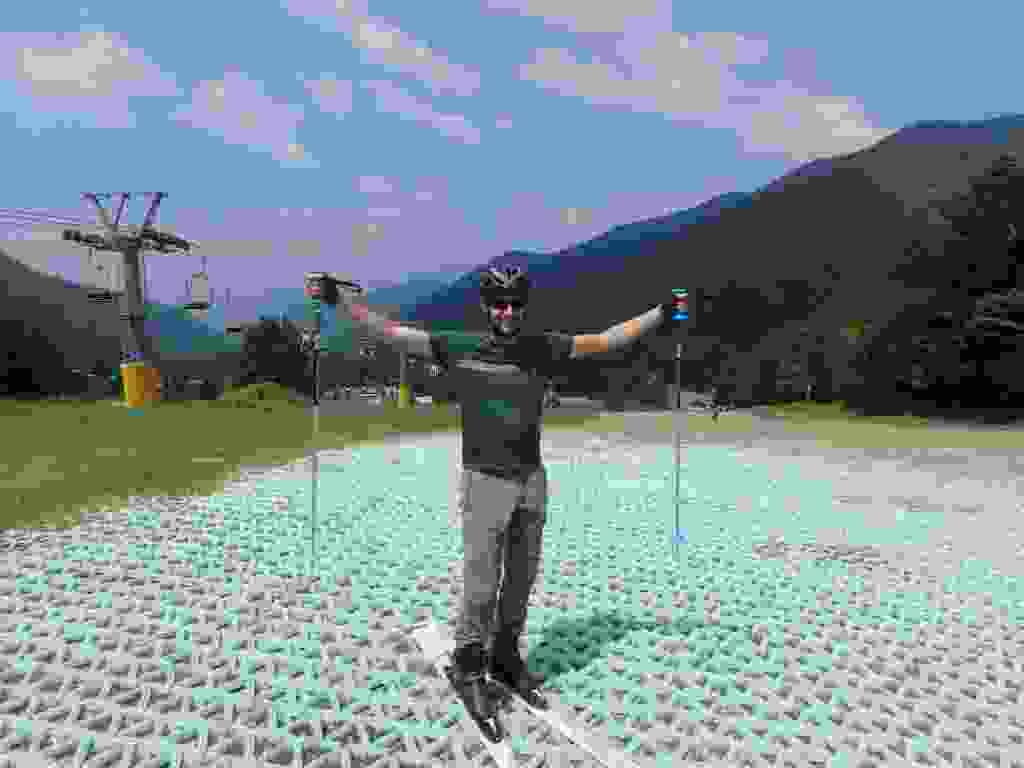
\includegraphics[width=\mywidth]{../wp-content/uploads/2015/08/P7315847-1024x768.jpg} } 
 \newline
 J'emprunte la route romantique japonaise qui ressemble à la route allemande du meme nom. \newline
 \newline
\centerline{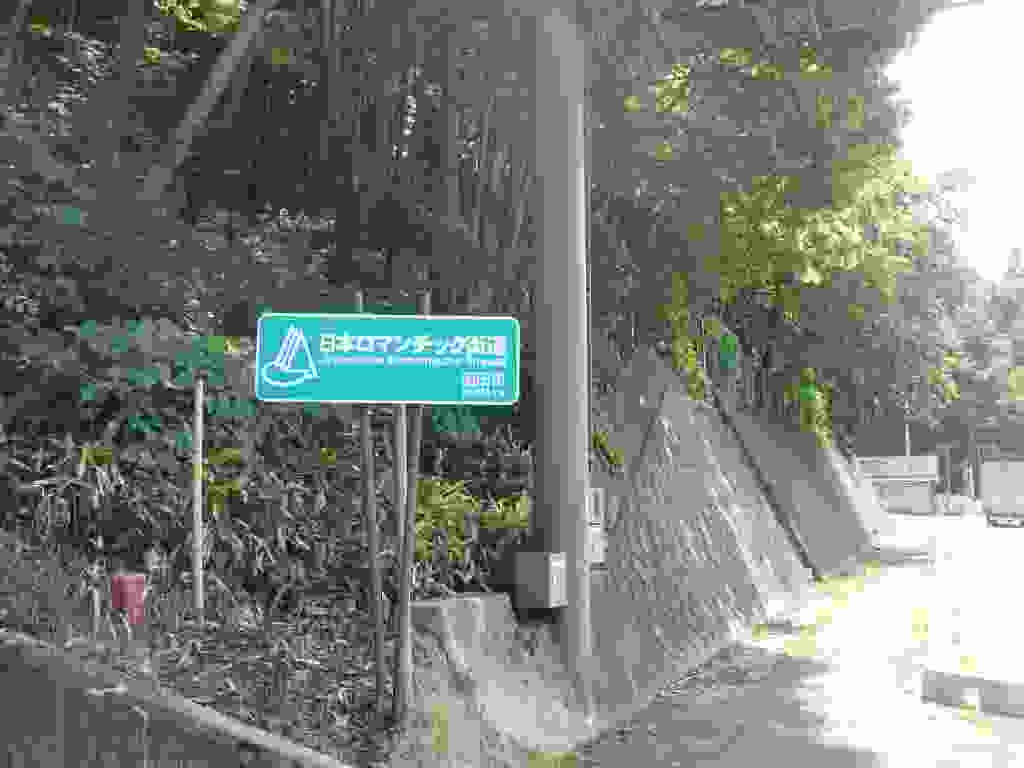
\includegraphics[width=\mywidth]{../wp-content/uploads/2015/08/P7315852-1024x768.jpg} } 
 \newline
 \newline
\centerline{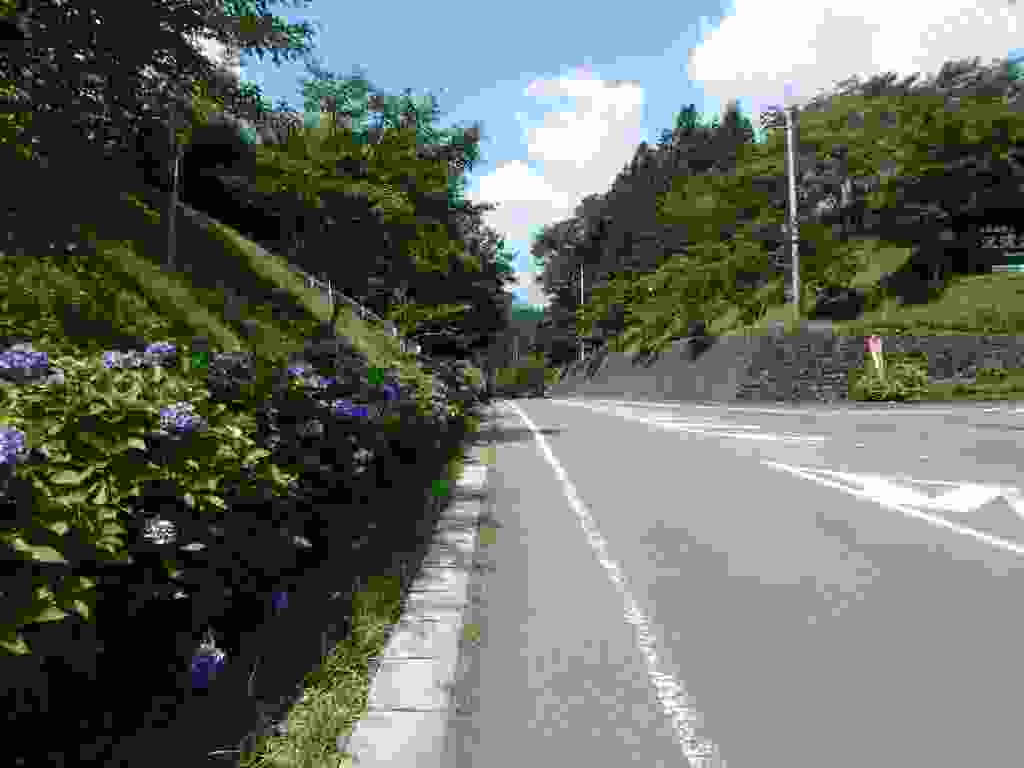
\includegraphics[width=\mywidth]{../wp-content/uploads/2015/08/P8015869-1024x768.jpg} } 
 \newline
 \newline
\centerline{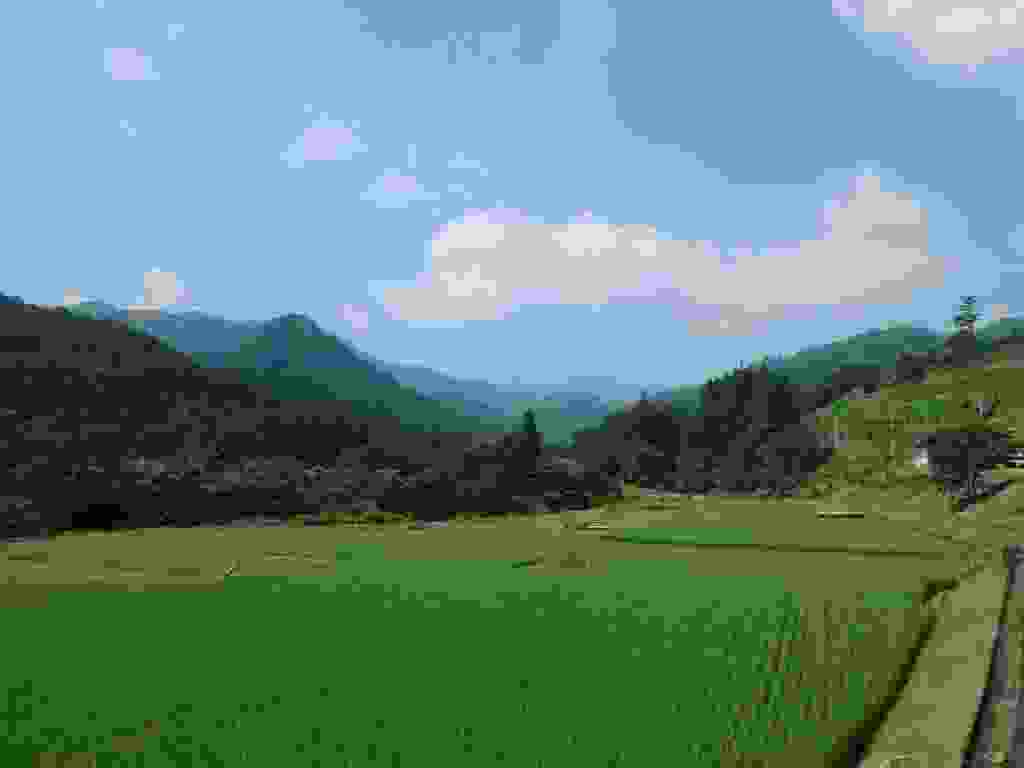
\includegraphics[width=\mywidth]{../wp-content/uploads/2015/08/P8015870-1024x768.jpg} } 
 \newline
 \newline
\centerline{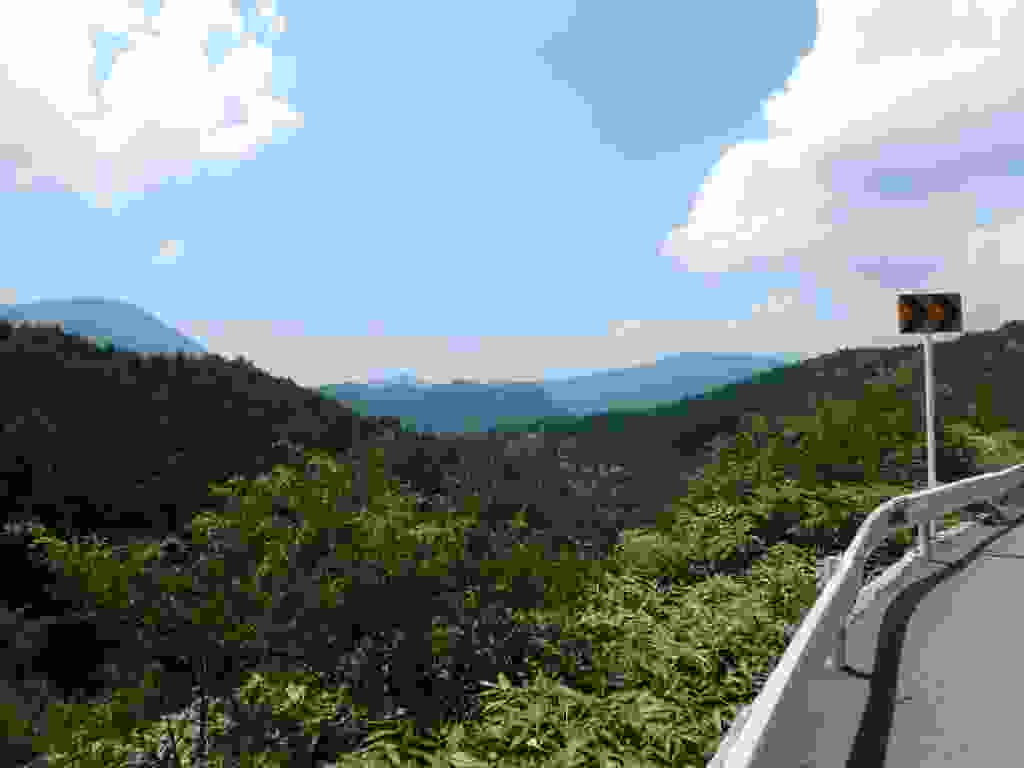
\includegraphics[width=\mywidth]{../wp-content/uploads/2015/08/P8025904-1024x768.jpg} } 
 \newline
 Pause pour aller voir la cascade de Fukiwari \newline
 \newline
\centerline{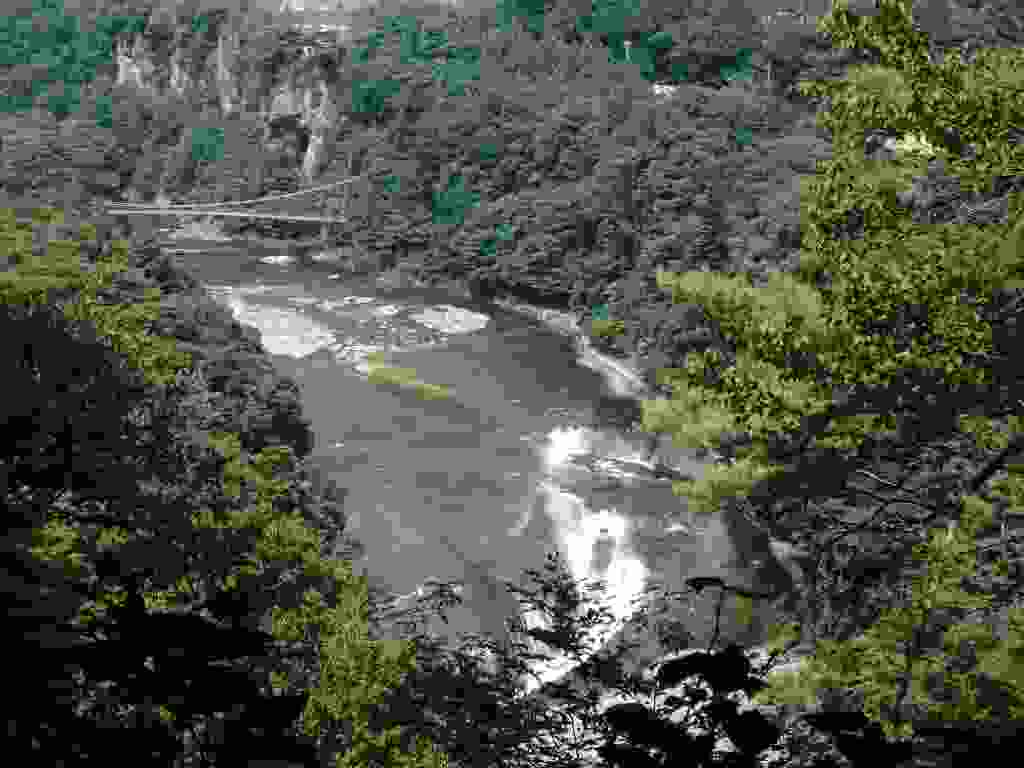
\includegraphics[width=\mywidth]{../wp-content/uploads/2015/08/P7315856-1024x768.jpg} } 
 \newline
 \newline
\centerline{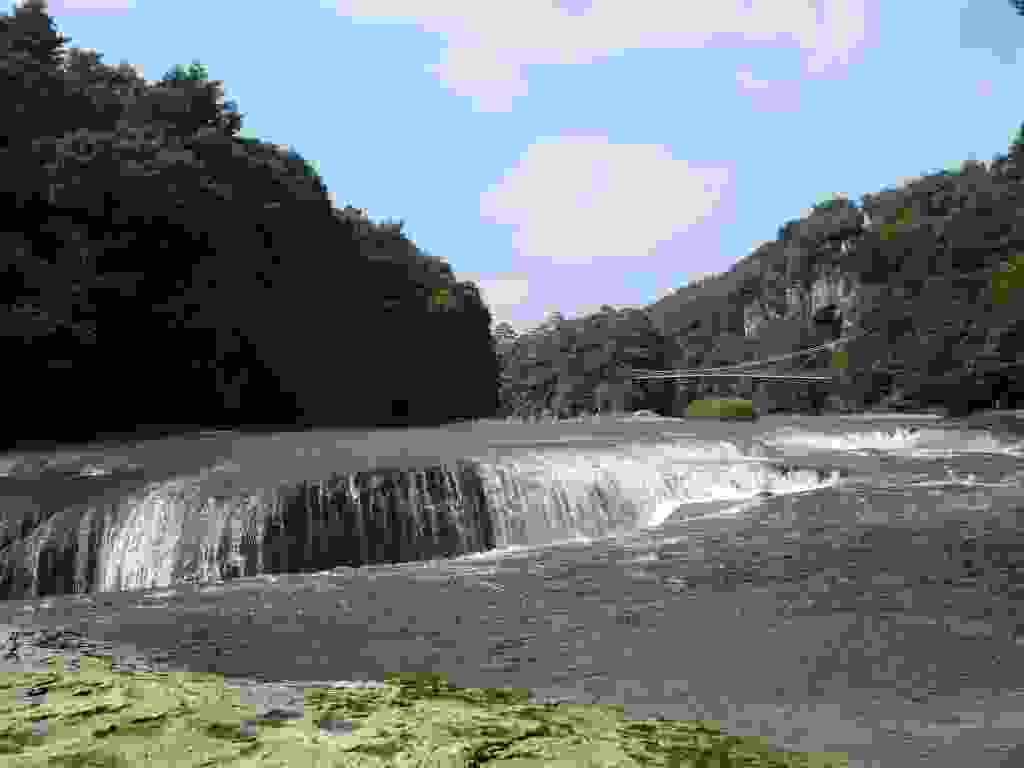
\includegraphics[width=\mywidth]{../wp-content/uploads/2015/08/P7315860-1024x768.jpg} } 
 \newline
 Je passe une soirée à Kusatsu, célèbre dans tout le Japon pour les vertus de son eau chaude naturelle. \newline
 \newline
\centerline{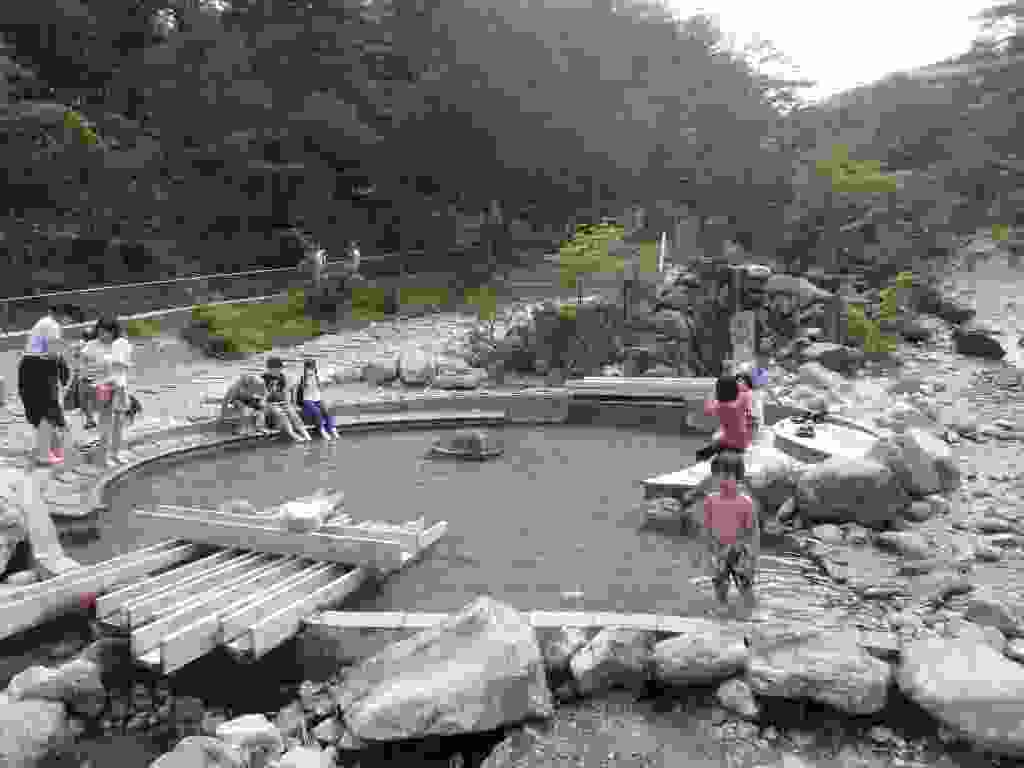
\includegraphics[width=\mywidth]{../wp-content/uploads/2015/08/P8015876-1024x768.jpg} } 
 \newline
 \newline
\centerline{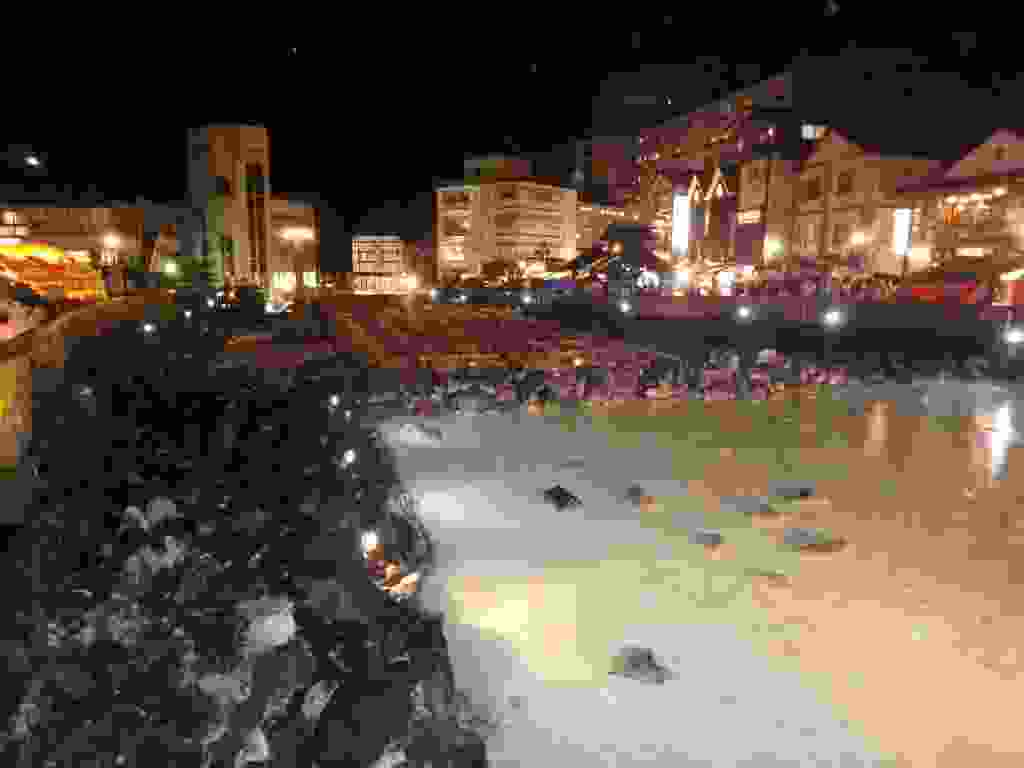
\includegraphics[width=\mywidth]{../wp-content/uploads/2015/08/P8015884-1024x768.jpg} } 
 \newline
 J'ai eu la chance d'y etre le jour d'un festival, avec une représentation dédiée à l'eau. \newline
 \newline
\centerline{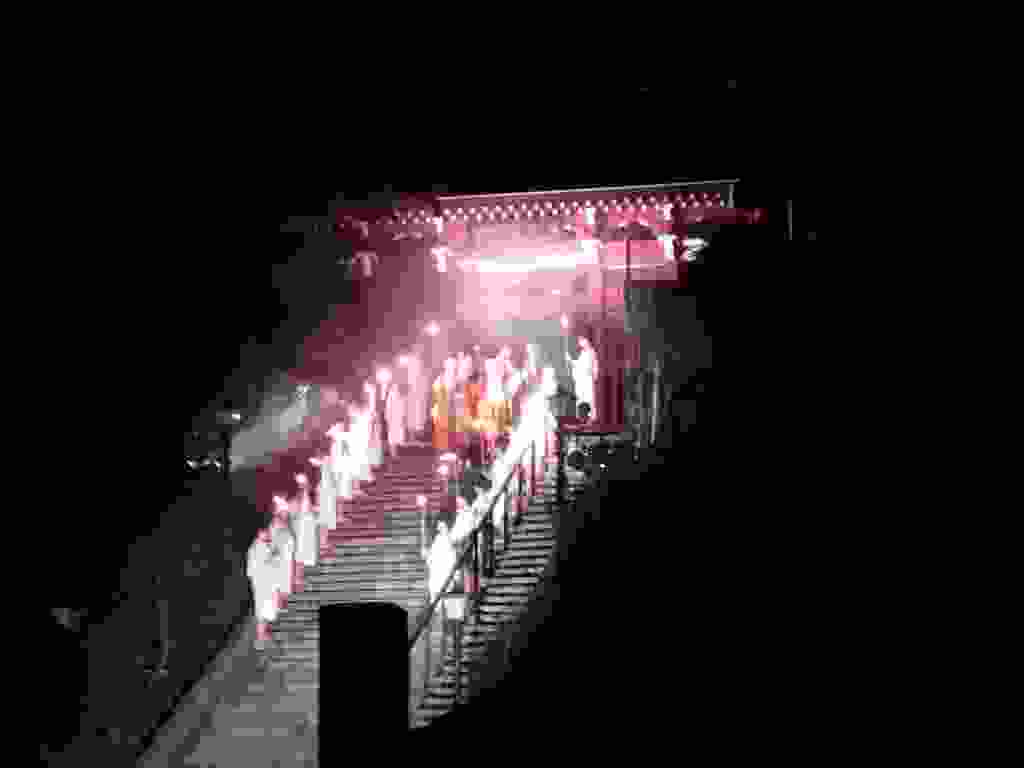
\includegraphics[width=\mywidth]{../wp-content/uploads/2015/08/P8015890-1024x768.jpg} } 
 \newline
 \newline
\centerline{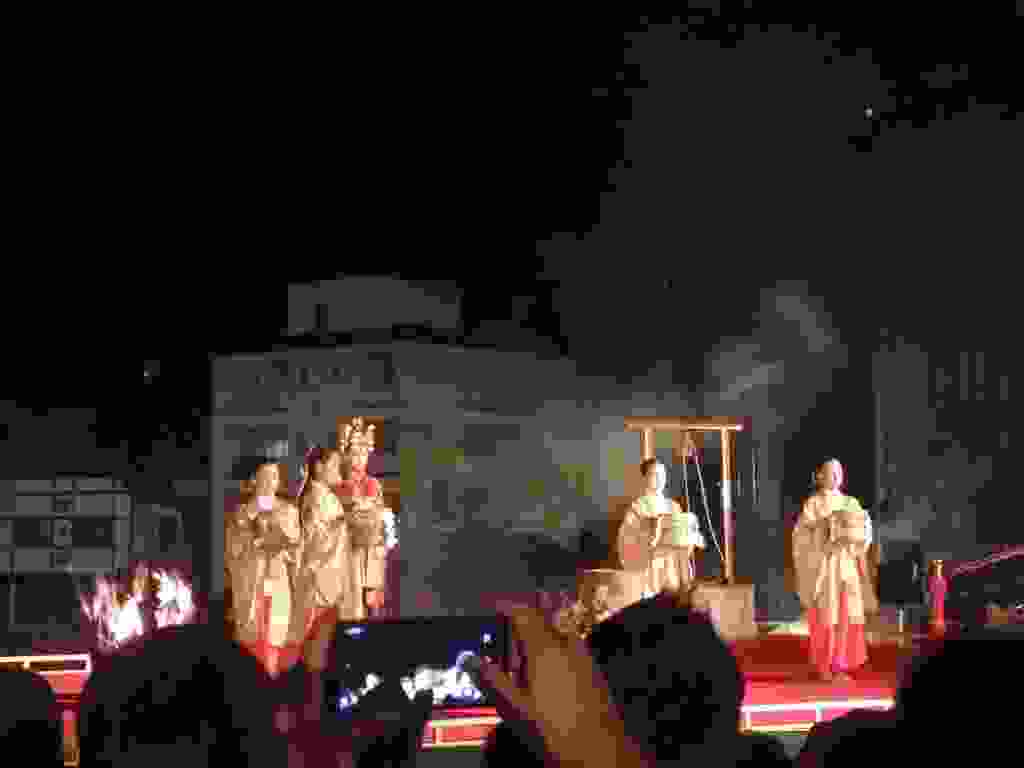
\includegraphics[width=\mywidth]{../wp-content/uploads/2015/08/P8015896-1024x768.jpg} } 
 \newline
 J'ai passé la nuit dans un hotel, voici le petit déjeuner japonais : \newline
 \newline
\centerline{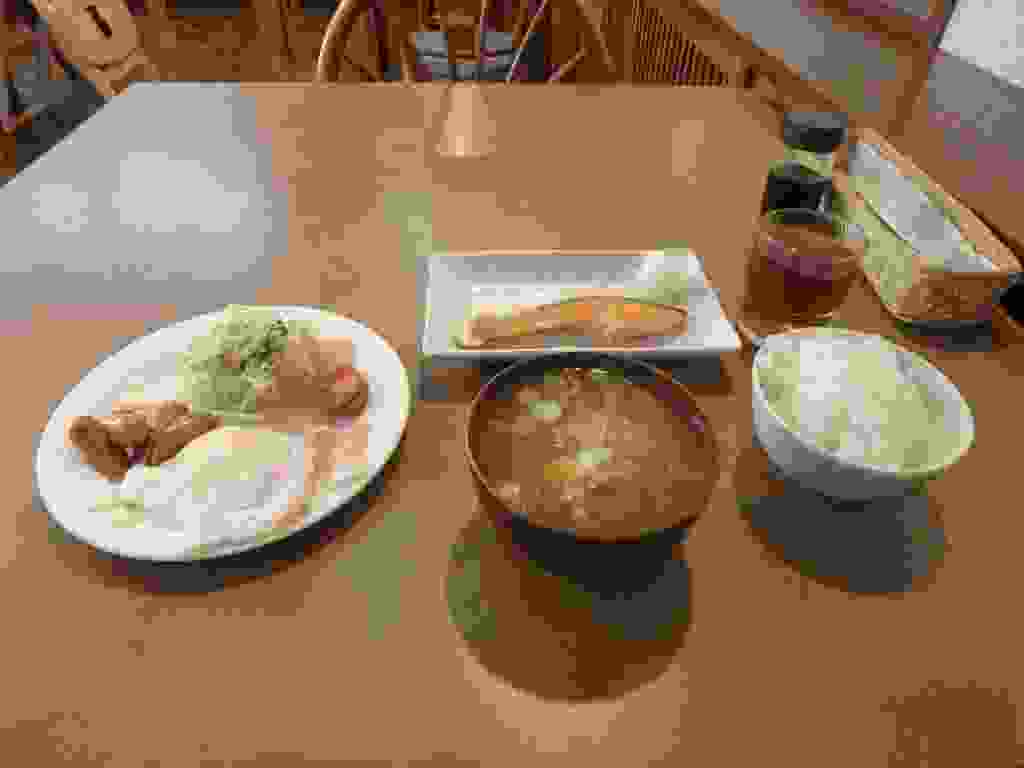
\includegraphics[width=\mywidth]{../wp-content/uploads/2015/08/P8025902-1024x768.jpg} } 
 \newline
 Enfin j'arrive à Nagano ou je visite le temple de Zenkoji, construit tout en bois. \newline
 \newline
\centerline{\includegraphics[width=\mywidth]{../wp-content/uploads/2015/08/P8025915-1024x768.jpg} } 
 \newline
 \newline
\centerline{\includegraphics[width=\mywidth]{../wp-content/uploads/2015/08/P8025925-1024x768.jpg} } 
 \newline
 \newline
\centerline{\includegraphics[width=\mywidth]{../wp-content/uploads/2015/08/P8025919-1024x768.jpg} } 
 \newline

\newpage
 
